% Contenido de la presentación del TP4 (Partes 1 y 2). Lo usan presentacion.tex y guion.tex.
% Cada diapositiva indica quién expone (\orador) y lo que dice (\note).

% =====================================================
% ---------- Portada ----------
% =====================================================
\begin{frame}[plain]
  \begin{tikzpicture}[remember picture, overlay]
    \node[anchor=east, xshift=1.2cm, yshift=-0.5cm, opacity=0.65] at (current page.east) {
      
\includegraphics[height=0.9\paperheight]{decoracion_a.png}
    };
    \fill[unc verde] (current page.north west) rectangle ([yshift=-1.6cm]current page.north east);
    \node[
      fill=unc verde, text=white, rounded corners=3pt,
      blur shadow={shadow blur steps=5, shadow xshift=0pt, shadow yshift=-3pt, shadow opacity=40},
      inner sep=12pt, minimum width=0.88\paperwidth, align=center, font=\Large\bfseries
    ] at ([yshift=-2.6cm]current page.north) {
      Sistemas de Radiocomunicación \\ Actividad 4: Fibra óptica
    };
    \node[anchor=center, text width=0.85\paperwidth, align=center] at ([yshift=-1.4cm]current page.center) {
      {\large\bfseries Parte 1: enlace punto a punto de 8 km\\Parte 2: red FTTH GPON para Marcos Juárez}\\[0.25cm]
      {\normalsize Arteaga Barrera, Cristian Eduardo\\Baccino, Luca\\ Mendes Rosa, Agustín\\ Monja, Ernesto Joaquín}\\[0.25cm]
      {\small Facultad de Ciencias Exactas, Físicas y Naturales -- Universidad Nacional de Córdoba}\\[0.15cm]
      {\small Córdoba, 2026}
    };
    \node[anchor=south] at ([yshift=0.1cm]current page.south) {
      
\includegraphics[height=1.2cm]{unc_fcefyn_logo.png}
    };
  \end{tikzpicture}
  \note{\textbf{Cristian Arteaga Barrera (apertura):} Buenas. Somos Cristian Arteaga Barrera, Luca Baccino, Agustín Mendes Rosa y Joaquín Monja, y vamos a presentar la Actividad 4 de fibra óptica: en la Parte 1, un enlace punto a punto de 8 km, y en la Parte 2, el diseño de una red FTTH GPON para Marcos Juárez.}
\end{frame}

% =====================================================
\section[Organización]{Organización}
\orador{Grupo Este}{Cristian Arteaga Barrera}
\begin{frame}{Organización de la exposición}
  \begin{columns}[T]
    \begin{column}{0.5\textwidth}
      \begin{block}{Grupo Este}
        \small
        \textbf{Arteaga Barrera}
        \begin{itemize}
          \item P1: planteo y selección de elementos
          \item P1: preguntas de análisis y conclusiones
          \item P2: investigación (REFEFO, videos, cables submarinos)
        \end{itemize}
        \textbf{Baccino}
        \begin{itemize}
          \item P1: presupuesto de potencia y gráficos
          \item P2: componentes, laboratorio, alcance
          \item P2: arquitectura y diseño de la Región Este
        \end{itemize}
      \end{block}
    \end{column}
    \begin{column}{0.5\textwidth}
      \setbeamercolor{block title}{bg=grupo oeste,fg=white}
      \setbeamercolor{block body}{bg=grupo oeste!8}
      \begin{block}{Grupo Oeste}
        \small
        \textbf{Mendes Rosa}
        \begin{itemize}
          \item P2: diseño de la Región Oeste y criterio de trazado del troncal
          \item P2: instituciones y plazas, fibras y puertos, cableado
        \end{itemize}
        \textbf{Monja}
        \begin{itemize}
          \item P2: conectividad mayorista con la calculadora de la cátedra
          \item P2: presupuesto óptico, televisión y conclusiones
        \end{itemize}
      \end{block}
    \end{column}
  \end{columns}
  \note{\textbf{Cristian Arteaga Barrera:} Nos dividimos en dos grupos, igual que en el trabajo. El Grupo Este, Luca y yo, presenta la Parte 1 completa y el comienzo de la Parte 2: la investigación, los componentes, el laboratorio, el alcance, la arquitectura y el diseño de la Región Este. El Grupo Oeste, Agustín y Joaquín, presenta el diseño de la Región Oeste y todo el dimensionamiento y la verificación de la red: instituciones, fibras, puertos, conectividad mayorista con la calculadora de la cátedra, presupuesto óptico y televisión.}
\end{frame}

% =====================================================
% ================= PARTE 1 ===========================
% =====================================================
\section[P1: Enlace P2P]{Parte 1: enlace P2P}
% Generado a partir de ../Parte_1/Presentacion/presentacion.tex con orador y guion.
\orador{Grupo Este}{Cristian Arteaga Barrera}
\begin{frame}{Planteo del problema}
  Interconectar dos edificios de un campus universitario mediante un enlace óptico punto a punto.

  \vspace{0.3cm}
  \begin{columns}[T]
    \begin{column}{0.5\textwidth}
      \textbf{Requerimientos}
      \begin{itemize}
        \item Distancia: \textbf{8 km}
        \item Velocidad: \textbf{1 Gbps} full dúplex
        \item Bidireccional con \textbf{dos fibras monomodo}
        \item Longitud de onda: \textbf{1310 nm}
        \item Tendido \textbf{subterráneo} con 2 cajas de empalme
      \end{itemize}
    \end{column}
    \begin{column}{0.5\textwidth}
      \textbf{Etapas del trabajo}
      \begin{enumerate}
        \item[A.] Selección de elementos
        \item[B.] Presupuesto de potencia
        \item[C.] Representación gráfica
        \item[D.] Preguntas de análisis
      \end{enumerate}
      \vspace{0.2cm}
      \textbf{Criterio:} cumplir técnicamente con la \textbf{opción más económica} que cubra el enlace.
    \end{column}
  \end{columns}
  \note{\textbf{Cristian Arteaga Barrera:} Arrancamos con la Parte 1: un enlace punto a punto de fibra entre dos edificios de un campus, a 8 km, a 1 Gbps full dúplex, con dos fibras monomodo a 1310 nm y tendido subterráneo con dos cajas de empalme. El trabajo tuvo cuatro etapas: elegir los elementos, hacer el presupuesto de potencia, representarlo gráficamente y responder las preguntas de análisis. El criterio que usamos en todo el trabajo fue cumplir técnicamente con la opción más económica.}
\end{frame}

\orador{Grupo Este}{Cristian Arteaga Barrera}
\begin{frame}{Transceptor: ProLabs SFP-1000BASE-LX-I-C}
  \begin{columns}[T]
    \begin{column}{0.52\textwidth}
      \begin{itemize}
        \item SFP 1000BASE-LX, 1310 nm, fibra monomodo
        \item Alcance de \textbf{10 km}, conector LC dúplex
        \item $-40$ a $85\,^\circ$C
      \end{itemize}
      \vspace{0.1cm}
      \begin{tabular}{lc}
        \toprule
        $P_t$ & $-9{,}5$ a $-3$ dBm \\
        $S_r$ (BER $10^{-12}$) & $-24$ dBm \\
        Sobrecarga & $0$ dBm \\
        \bottomrule
      \end{tabular}
      \vspace{0.2cm}
      \begin{block}{Optical Budget (peor caso)}
        \centering
        $OB = P_{t,min} - S_r = -9{,}5 - (-24) = \mathbf{14{,}5\ dB}$
      \end{block}
    \end{column}
    \begin{column}{0.48\textwidth}
      \centering
      \textbf{Precios de referencia}\\[0.1cm]
      \small
      \begin{tabular}{lcc}
        \toprule
        \textbf{Tipo} & \textbf{Alcance} & \textbf{US\$} \\
        \midrule
        LX 1310 nm & 10 km & 8 \\
        LX 1310 nm & 20 km & 8 \\
        EX 1310 nm & 40 km & 16 \\
        EX 1550 nm & 40 km & 27 \\
        ZX 1550 nm & 80 km & 27 \\
        \bottomrule
      \end{tabular}\\[0.2cm]
      \normalsize La categoría de 10 km es la \textbf{más económica} que cubre los 8 km y no necesita atenuadores.
    \end{column}
  \end{columns}
  \note{\textbf{Cristian Arteaga Barrera:} Para el transceptor elegimos un SFP 1000BASE-LX de ProLabs, a 1310 nm, con alcance de 10 km. Lo importante son tres números: potencia de transmisión mínima de -9,5 dBm, sensibilidad de -24 dBm y sobrecarga de 0 dBm. Con eso el optical budget en el peor caso es de 14,5 dB. En la tabla de precios se ve que la categoría de 10 km es la más barata que cubre los 8 km, y además no necesita atenuadores.}
\end{frame}

\orador{Grupo Este}{Cristian Arteaga Barrera}
\begin{frame}{Fibra: G.652.D frente a G.657}
  \begin{columns}[T]
    \begin{column}{0.5\textwidth}
      \textbf{G.652.D}
      \begin{itemize}
        \item Monomodo estándar, bajo pico de agua
        \item Fibra de uso general en redes troncales
        \item 12 a 17 US\$/km
      \end{itemize}
    \end{column}
    \begin{column}{0.5\textwidth}
      \textbf{G.657.A}
      \begin{itemize}
        \item Insensible a curvaturas pronunciadas
        \item Pensada para instalaciones internas y FTTH
        \item 16,5 a 33 US\$/km (A1 y A2)
      \end{itemize}
    \end{column}
  \end{columns}
  \vspace{0.4cm}
  \begin{block}{Elección: G.652.D}
    Ambas tienen una atenuación similar en 1310 nm. En un tramo troncal en ducto los radios de curvatura son amplios, así que la ventaja de la G.657 no justifica su mayor costo.
  \end{block}
  \note{\textbf{Cristian Arteaga Barrera:} Para la fibra comparamos G.652.D con G.657.A. A 1310 nm las dos atenúan prácticamente lo mismo; la G.657 tiene la ventaja de tolerar curvaturas cerradas, que sirve en instalaciones internas o FTTH. En un tramo troncal en ducto los radios de curvatura son amplios, así que esa ventaja no justifica su mayor costo. Por eso elegimos G.652.D.}
\end{frame}

\orador{Grupo Este}{Cristian Arteaga Barrera}
\begin{frame}{Cable: Lightera CFOA-SM-DDR-S 04F TS G-652D}
  \begin{columns}[T]
    \begin{column}{0.55\textwidth}
      \begin{itemize}
        \item Dieléctrico, para \textbf{ductos}, núcleo totalmente seco
        \item Capa de fibra de vidrio contra \textbf{roedores}
        \item \textbf{4 fibras}: 2 en uso y 2 de reserva
        \item Diámetro de 12,4 mm
        \item Bobinas de \textbf{4000 m}: los 8 km requieren empalmes intermedios
      \end{itemize}
    \end{column}
    \begin{column}{0.45\textwidth}
      \begin{block}{Atenuación adoptada}
        \centering
        $\alpha = 0{,}38$ dB/km a 1310 nm
      \end{block}
      \small
      Se usa la atenuación máxima de fibra G.652.D cableada de Lightera.
    \end{column}
  \end{columns}
  \vspace{0.3cm}
  \small Fabricado según ABNT NBR 14773. En Argentina, la norma de referencia para cables exteriores es la IRAM 4225.
  \note{\textbf{Cristian Arteaga Barrera:} El cable es el Lightera CFOA-SM-DDR-S de 4 fibras: dieléctrico, para ductos, de núcleo seco y con protección contra roedores. Usamos 2 fibras y dejamos 2 de reserva. Viene en bobinas de 4 km, por lo que los 8 km necesitan empalmes intermedios. Para el cálculo adoptamos 0,38 dB/km, que es la atenuación máxima que da Lightera para G.652.D cableada. En Argentina la norma de referencia para cables exteriores es la IRAM 4225.}
\end{frame}

\orador{Grupo Este}{Cristian Arteaga Barrera}
\begin{frame}{Conectores, empalmes y ODF}
  \begin{columns}[T]
    \begin{column}{0.52\textwidth}
      \textbf{Por fibra (un sentido)}\\[0.1cm]
      \small
      \begin{tabular}{lcc}
        \toprule
        \textbf{Elemento} & \textbf{Cant.} & \textbf{Pérdida} \\
        \midrule
        Fibra G.652.D & 8 km & 0,38 dB/km \\
        Patchcord LC/UPC & 2 & 0,4 dB \\
        Pigtail LC/UPC & 2 & 0,2 dB \\
        Adaptador de panel & 2 & 0,2 dB \\
        Empalme por fusión & 4 & 0,1 dB \\
        \bottomrule
      \end{tabular}\\[0.15cm]
      \normalsize
      \footnotesize Valores típicos del apunte de la cátedra.
    \end{column}
    \begin{column}{0.48\textwidth}
      \textbf{ODF: Lightera DIO BW12}
      \begin{itemize}
        \item Hasta 12 empalmes y 12 adaptadores LC dúplex
        \item Admite cables \emph{loose tube} de hasta 14 mm
        \item Montaje en rack de 19 pulgadas o en pared
        \item Es el modelo de \textbf{menor capacidad} que admite el cable de 4 fibras
      \end{itemize}
    \end{column}
  \end{columns}
  \note{\textbf{Cristian Arteaga Barrera:} Esta tabla resume todos los eventos de pérdida de una fibra en un sentido: la fibra, dos patchcords, dos pigtails, dos adaptadores de panel y cuatro empalmes por fusión, con los valores típicos del apunte de la cátedra. Para terminar los cables usamos el ODF Lightera DIO BW12, que es el de menor capacidad que admite el cable de 4 fibras. Con esto le paso a Luca, que va a mostrar el presupuesto de potencia.}
\end{frame}

\orador{Grupo Este}{Luca Baccino}
\begin{frame}{Ecuaciones del presupuesto}
  \begin{columns}[T]
    \begin{column}{0.5\textwidth}
      \textbf{Pérdida total}
      \[ A_{total} = A_f \cdot L + P_c + P_{em} \]
      \textbf{Potencia recibida}
      \[ P_r = P_t - A_{total} \]
      \textbf{Condición de viabilidad}
      \[ P_t - S_r \geq A_{total} + M_s \]
    \end{column}
    \begin{column}{0.5\textwidth}
      \begin{itemize}
        \item Se calcula con $P_{t,min}$ y la atenuación máxima de la fibra (peor caso).
        \item Margen de seguridad $M_s = 3$ dB: mínimo del rango de 3 a 6 dB recomendado por la cátedra.
      \end{itemize}
    \end{column}
  \end{columns}
  \note{\textbf{Luca Baccino:} Gracias, Cristian. El presupuesto se arma con tres ecuaciones: la pérdida total es la fibra por la longitud más conectores y empalmes; la potencia recibida es la transmitida menos esa pérdida; y el enlace es viable si la diferencia entre la potencia transmitida y la sensibilidad cubre la pérdida total más el margen de seguridad. Calculamos siempre en el peor caso, con la potencia mínima del transmisor y la atenuación máxima de la fibra, y usamos un margen de 3 dB, el mínimo del rango que recomienda la cátedra.}
\end{frame}

\orador{Grupo Este}{Luca Baccino}
\begin{frame}{Cálculo de las pérdidas}
  \begin{columns}[c]
    \begin{column}{0.55\textwidth}
      \begin{align*}
        A_{fibra} &= 0{,}38 \times 8 = 3{,}04 \text{ dB} \\[0.1cm]
        P_c &= 2(0{,}4) + 2(0{,}2) + 2(0{,}2) = 1{,}60 \text{ dB} \\[0.1cm]
        P_{em} &= 4 \times 0{,}1 = 0{,}40 \text{ dB} \\[0.1cm]
        \hline
        A_{total} &= \mathbf{5{,}04 \text{ dB}}
      \end{align*}
    \end{column}
    \begin{column}{0.45\textwidth}
      \centering
      \begin{tikzpicture}
        \begin{axis}[
          xbar stacked, width=\textwidth, height=3.6cm,
          xmin=0, xmax=5.5, ytick=\empty, axis y line=none,
          xlabel={Pérdida [dB]}, tick label style={font=\scriptsize},
          label style={font=\scriptsize}, bar width=0.6cm,
          legend style={font=\scriptsize, at={(0.5,-0.55)}, anchor=north, legend columns=1, draw=none},
          area legend
        ]
          \addplot[fill=unc verde, draw=none] coordinates {(3.04,0)};
          \addplot[fill=unc verdeclaro, draw=none] coordinates {(1.6,0)};
          \addplot[fill=orange!80, draw=none] coordinates {(0.4,0)};
          \legend{Fibra (60\,\%), Conexiones (32\,\%), Empalmes (8\,\%)}
        \end{axis}
      \end{tikzpicture}
    \end{column}
  \end{columns}
  \vspace{0.3cm}
  La \textbf{fibra} concentra la mayor parte de la pérdida: la distancia es la variable que más pesa en el presupuesto.
  \note{\textbf{Luca Baccino:} La fibra aporta 3,04 dB, las conexiones 1,6 dB y los empalmes 0,4 dB: en total 5,04 dB. En el gráfico se ve que la fibra concentra el 60 por ciento de la pérdida, así que en este enlace la variable que más pesa es la distancia.}
\end{frame}

\orador{Grupo Este}{Luca Baccino}
\begin{frame}{Resultado: el enlace es viable}
  \begin{columns}[T]
    \begin{column}{0.5\textwidth}
      \begin{tabular}{lr}
        \toprule
        $P_{t,min}$ & $-9{,}50$ dBm \\
        $A_{total}$ & $5{,}04$ dB \\
        $P_{r,min}$ & $-14{,}54$ dBm \\
        $S_r$ & $-24{,}00$ dBm \\
        $P_{r,min} - S_r$ & $9{,}46$ dB \\
        $M_s$ & $3{,}00$ dB \\
        \textbf{Margen sobrante} & $6{,}46$ dB \\
        \bottomrule
      \end{tabular}
    \end{column}
    \begin{column}{0.5\textwidth}
      \begin{block}{Condición de viabilidad}
        \centering
        $OB = 14{,}5 \geq 5{,}04 + 3 = 8{,}04$ dB \checkmark
      \end{block}
      \begin{block}{Sobrecarga del receptor}
        \centering
        $P_{r,max} = -3 - 5{,}04 = -8{,}04$ dBm $< 0$ dBm \checkmark
      \end{block}
      \small Aun con $M_s = 6$ dB quedarían 3,46 dB de holgura.
    \end{column}
  \end{columns}
  \note{\textbf{Luca Baccino:} Con -9,5 dBm transmitidos y 5,04 dB de pérdida llegan -14,54 dBm, contra una sensibilidad de -24 dBm. Descontando los 3 dB de margen todavía sobran 6,46 dB, así que el enlace es viable. También verificamos el otro extremo: con la potencia máxima llegan -8,04 dBm, por debajo de la sobrecarga de 0 dBm, así que no hace falta atenuador. Incluso con un margen de 6 dB sobraría potencia.}
\end{frame}

\orador{Grupo Este}{Luca Baccino}
\begin{frame}{Verificación de la dispersión cromática}
  \begin{columns}[T]
    \begin{column}{0.52\textwidth}
      \begin{itemize}
        \item G.652: $\lambda_0 = 1300$ a $1324$ nm, $S_0 \leq 0{,}092$ ps/(nm$^2\cdot$km)
        \[ D(\lambda) = \frac{S_0}{4}\left(\lambda - \frac{\lambda_0^4}{\lambda^3}\right) \]
        \item Peor caso en el rango del láser (1270 a 1355 nm): $|D| = 5{,}29$ ps/(nm$\cdot$km)
        \item Ancho espectral RMS del láser LX: $\sigma_\lambda = 4$ nm
      \end{itemize}
    \end{column}
    \begin{column}{0.48\textwidth}
      \[ \Delta\tau = |D| \cdot L \cdot \sigma_\lambda = 169 \text{ ps} \]
      \[ B \cdot \Delta\tau = 1{,}25\text{ Gbps} \times 169 \text{ ps} = 0{,}21 \]
      \begin{block}{Criterio $B \cdot \Delta\tau \leq 0{,}25$ \checkmark}
        El enlace está limitado por \textbf{atenuación}, no por dispersión.
      \end{block}
    \end{column}
  \end{columns}
  \note{\textbf{Luca Baccino:} Además de la potencia verificamos la dispersión cromática. Con los parámetros de la G.652 y el rango de longitudes de onda del láser, el peor coeficiente es de 5,29 ps por nm y km. Con el ancho espectral del láser LX, el ensanchamiento del pulso es de 169 ps, y el producto con la tasa de bits da 0,21, por debajo del criterio de 0,25. Conclusión: el enlace está limitado por atenuación y no por dispersión.}
\end{frame}

\orador{Grupo Este}{Luca Baccino}
\begin{frame}{Esquema del enlace (una fibra, A $\rightarrow$ B)}
  \centering
  \resizebox{\textwidth}{!}{%
    \begin{tikzpicture}[font=\footnotesize,
        router/.style={draw, thick, rounded corners=2pt, minimum width=2.6cm, minimum height=2.0cm, fill=blue!4},
        sfp/.style={draw, thick, rounded corners=2pt, minimum width=1.4cm, minimum height=1.2cm, align=center, fill=blue!15},
        odf/.style={draw, thick, minimum width=4.4cm, minimum height=2.0cm, fill=gray!12},
        adaptador/.style={draw, thick, minimum width=1.4cm, minimum height=0.5cm, fill=gray!35},
        caja/.style={draw, thick, rounded corners=5pt, minimum width=1.2cm, minimum height=0.8cm, fill=orange!15},
        empalme/.style={circle, fill=red!75!black, inner sep=1.7pt},
        conector/.style={draw, thick, fill=white, minimum width=0.24cm, minimum height=0.24cm, inner sep=0pt},
        perdida/.style={font=\scriptsize\bfseries, text=red!75!black},
        nombre/.style={font=\scriptsize, text=black!70},
        potencia/.style={draw=blue!60!black, thick, rounded corners=2pt, fill=white, font=\scriptsize, align=left, inner sep=3pt},
        evento/.style={circle, draw=black!60, fill=white, font=\tiny, inner sep=0.6pt, minimum size=0.36cm}]

        % ---------- Sitio A: Router, SFP y ODF ----------
        \node[router] (RA) at (1.3,0) {};
        \node[font=\footnotesize\bfseries, above] at (RA.north) {Router A};
        \node[sfp] (SA) at (1.9,0) {\textbf{SFP}\\[1pt]TX};

        \node[odf] (OA) at (6.6,0) {};
        \node[font=\footnotesize\bfseries, above] at (OA.north) {ODF A};

        % ---------- Sitio B: ODF, SFP y Router ----------
        \node[odf] (OB) at (16.6,0) {};
        \node[font=\footnotesize\bfseries, above] at (OB.north) {ODF B};
        \node[router] (RB) at (21.9,0) {};
        \node[font=\footnotesize\bfseries, above] at (RB.north) {Router B};
        \node[sfp] (SB) at (21.3,0) {\textbf{SFP}\\[1pt]RX};

        % ---------- Potencias del SFP TX y del SFP RX ----------
        \node[potencia, anchor=north] (PA) at (1.9,-1.25) {%
            $P_{t,\mathrm{min}} = -9{,}5$ dBm\\
            $P_{t,\mathrm{max}} = -3$ dBm};
        \draw[-{Stealth}, thick, blue!60!black] (SA.south) -- (PA.north);

        \node[potencia, anchor=north] (PB) at (21.3,-1.25) {%
            $P_{r,\mathrm{min}} = -14{,}54$ dBm\\
            $P_{r,\mathrm{max}} = -8{,}04$ dBm\\
            $S_r = -24$ dBm};
        \draw[{Stealth}-, thick, blue!60!black] (SB.south) -- (PB.north);

        % ---------- Fibras: patchcord (azul), pigtail (amarillo) y cable (gris) ----------
        \draw[line width=1.6pt, blue!60!black] (2.6,0) -- (5.0,0);     % patchcord A
        \draw[line width=1.6pt, yellow!55!black] (6.4,0) -- (8.0,0);   % pigtail A
        \draw[line width=2.6pt, black!65] (8.0,0) -- (15.2,0);         % cable exterior
        \draw[line width=1.6pt, yellow!55!black] (15.2,0) -- (16.8,0); % pigtail B
        \draw[line width=1.6pt, blue!60!black] (18.2,0) -- (20.6,0);   % patchcord B

        % ---------- Adaptadores de panel (acoplan patchcord con pigtail) ----------
        \node[adaptador] (AA) at (5.7,0) {};
        \node[adaptador] (AB) at (17.5,0) {};

        % ---------- Cajas de empalme ----------
        \node[caja] (C1) at (10.4,0) {};
        \node[font=\footnotesize\bfseries, above=1pt] at (C1.north) {Caja 1};
        \node[caja] (C2) at (12.8,0) {};
        \node[font=\footnotesize\bfseries, above=1pt] at (C2.north) {Caja 2};

        % ---------- Conectores LC/UPC ----------
        \node[conector] at (2.6,0) {};
        \node[conector] at (5.0,0) {};
        \node[conector] at (6.4,0) {};
        \node[conector] at (16.8,0) {};
        \node[conector] at (18.2,0) {};
        \node[conector] at (20.6,0) {};

        % ---------- Empalmes por fusión (pigtail - cable) ----------
        \node[empalme] at (8.0,0) {};
        \node[empalme] at (10.4,0) {};
        \node[empalme] at (12.8,0) {};
        \node[empalme] at (15.2,0) {};

        % ---------- Nombres de los elementos del ODF ----------
        \node[nombre] at (3.8,0.75) {Patchcord};
        \node[nombre] at (5.7,0.75) {Adaptador};
        \node[nombre] at (7.2,0.75) {Pigtail};
        \node[nombre] at (16.0,0.75) {Pigtail};
        \node[nombre] at (17.5,0.75) {Adaptador};
        \node[nombre] at (19.4,0.75) {Patchcord};

        % ---------- Pérdida (arriba) y número de evento (abajo) ----------
        \foreach \x/\p/\n in {3.8/0{,}4/1, 5.7/0{,}2/2, 7.2/0{,}2/3, 8.0/0{,}1/4,
                              9.2/1{,}01/5, 11.6/1{,}01/7, 14.0/1{,}01/9,
                              15.2/0{,}1/10, 16.0/0{,}2/11, 17.5/0{,}2/12, 19.4/0{,}4/13}{
            \node[perdida] at (\x,0.4) {$\p$};
            \node[evento] at (\x,-0.45) {\n};
        }
        \foreach \x/\n in {10.4/6, 12.8/8}{
            \node[perdida] at (\x,-0.62) {$0{,}1$};
            \node[evento] at (\x+0.45,-0.62) {\n};
        }

        % ---------- Eje de distancia acumulada ----------
        \draw[-{Stealth}, thick] (8.0,-1.45) -- (15.8,-1.45) node[right, font=\scriptsize] {$d$ [km]};
        \foreach \x/\d in {8.0/0{,}00, 10.4/2{,}67, 12.8/5{,}33, 15.2/8{,}00}{
            \draw[thick] (\x,-1.35) -- (\x,-1.55);
            \node[below, font=\scriptsize] at (\x,-1.55) {$\d$};
        }
        \foreach \x in {8.0, 15.2}{
            \draw[densely dotted, black!50] (\x,-1.35) -- (\x,-0.7);
        }
        \foreach \x in {10.4, 12.8}{
            \draw[densely dotted, black!50] (\x,-1.35) -- (\x,-0.85);
        }

        % ---------- Referencias ----------
        \node[conector] at (0.5,-3.7) {};
        \node[right, font=\scriptsize] at (0.65,-3.7) {Conector LC/UPC};
        \node[adaptador, minimum width=0.6cm, minimum height=0.3cm] at (5.0,-3.7) {};
        \node[right, font=\scriptsize] at (5.4,-3.7) {Adaptador de panel LC/UPC};
        \node[empalme] at (10.6,-3.7) {};
        \node[right, font=\scriptsize] at (10.75,-3.7) {Empalme por fusión};
        \node[evento] at (15.5,-3.7) {n};
        \node[right, font=\scriptsize] at (15.7,-3.7) {N° de evento};

        \draw[line width=1.6pt, blue!60!black] (0.2,-4.4) -- (0.8,-4.4);
        \node[right, font=\scriptsize] at (0.8,-4.4) {Patchcord LC/UPC};
        \draw[line width=1.6pt, yellow!55!black] (5.0,-4.4) -- (5.6,-4.4);
        \node[right, font=\scriptsize] at (5.7,-4.4) {Pigtail LC/UPC};
        \draw[line width=2.6pt, black!65] (10.3,-4.4) -- (10.9,-4.4);
        \node[right, font=\scriptsize] at (11.0,-4.4) {Cable CFOA-SM-DDR-S 04F};
    \end{tikzpicture}%
    }

  \vspace{0.4cm}
  \small
  \begin{itemize}
    \item Pérdidas en dB (en rojo). Los elementos internos de cada sitio están fuera de escala.
    \item Se suponen 3 tramos iguales de 2,67 km, cada uno menor que una bobina de 4 km.
  \end{itemize}
  \note{\textbf{Luca Baccino:} Este es el esquema de una fibra de A a B. Se ve cada elemento con su pérdida en rojo y numerado como evento: patchcord, adaptador, pigtail, empalme, los tres tramos de cable de 2,67 km con las dos cajas de empalme, y lo mismo del lado B. Abajo está el eje de distancia acumulada y en los extremos las potencias del transmisor y del receptor. Los elementos internos de cada sitio están fuera de escala.}
\end{frame}

\orador{Grupo Este}{Luca Baccino}
\begin{frame}{Gráfico del presupuesto óptico}
  \centering
  \begin{tikzpicture}
    \begin{axis}[
        width=\textwidth, height=0.82\textheight,
        xmin=-1.5, xmax=11.4, ymin=-26, ymax=-1,
        xlabel={Distancia acumulada [km]},
        ylabel={Potencia óptica [dBm]},
        xtick={0,2.667,5.333,8}, xticklabels={$0{,}00$,$2{,}67$,$5{,}33$,$8{,}00$},
        ytick={-24,-20,-16,-12,-8,-4},
        grid=major, grid style={black!12},
        tick label style={font=\scriptsize},
        label style={font=\scriptsize},
        clip=false,
        legend style={font=\tiny, at={(axis cs:0.3,-15.2)}, anchor=north west, fill=white, fill opacity=0.9, text opacity=1},
        legend cell align=left
    ]
        \fill[blue!5] (axis cs:-1.5,-26) rectangle (axis cs:0,-1);
        \fill[blue!5] (axis cs:8,-26) rectangle (axis cs:9.5,-1);
        \node[font=\tiny, align=center] at (axis cs:-0.75,-2.2) {Sitio A};
        \node[font=\tiny, align=center] at (axis cs:8.75,-2.2) {Sitio B};

        \addplot[very thick, blue!70!black, mark=none] coordinates {
            (-1.2,-9.50) (-0.9,-9.50) (-0.9,-9.90) (-0.6,-9.90) (-0.6,-10.10)
            (-0.3,-10.10) (-0.3,-10.30) (0,-10.30) (0,-10.40)
            (2.667,-11.413) (2.667,-11.513) (5.333,-12.527) (5.333,-12.627)
            (8,-13.640) (8,-13.740) (8.3,-13.740) (8.3,-13.940) (8.6,-13.940)
            (8.6,-14.140) (8.9,-14.140) (8.9,-14.540) (9.2,-14.540)};
        \addlegendentry{Nivel con $P_{t,min} = -9{,}5$ dBm}

        \addplot[thick, dashed, black!55, mark=none] coordinates {
            (-1.2,-3.00) (-0.9,-3.00) (-0.9,-3.40) (-0.6,-3.40) (-0.6,-3.60)
            (-0.3,-3.60) (-0.3,-3.80) (0,-3.80) (0,-3.90)
            (2.667,-4.913) (2.667,-5.013) (5.333,-6.027) (5.333,-6.127)
            (8,-7.140) (8,-7.240) (8.3,-7.240) (8.3,-7.440) (8.6,-7.440)
            (8.6,-7.640) (8.9,-7.640) (8.9,-8.040) (9.2,-8.040)};
        \addlegendentry{Nivel con $P_{t,max} = -3$ dBm}

        \addplot[thick, red, dashed, domain=-1.5:9.5, samples=2] {-24};
        \addlegendentry{Sensibilidad $S_r = -24$ dBm}
        \addplot[very thick, orange, dotted, domain=-1.5:9.5, samples=2] {-21};
        \addlegendentry{Umbral de diseño $S_r + M_s = -21$ dBm}

        \node[circle, fill=blue!70!black, inner sep=1.3pt] at (axis cs:-1.2,-9.5) {};
        \node[font=\tiny, above right, fill=white, inner sep=1pt] at (axis cs:-1.25,-9.3) {$P_{t} = -9{,}5$};
        \node[circle, fill=blue!70!black, inner sep=1.3pt] at (axis cs:9.2,-14.54) {};
        \node[font=\tiny, below left] at (axis cs:9.2,-14.54) {$P_{r} = -14{,}54$};

        \draw[{Stealth}-{Stealth}, thick, blue!70!black] (axis cs:9.75,-9.5) -- (axis cs:9.75,-14.54)
            node[midway, right, font=\tiny, align=left] {$\Sigma$ pérdidas\\$5{,}04$ dB};
        \draw[densely dotted, blue!70!black] (axis cs:-1.2,-9.5) -- (axis cs:9.75,-9.5);
        \draw[{Stealth}-{Stealth}, thick, green!50!black] (axis cs:9.75,-14.54) -- (axis cs:9.75,-21)
            node[midway, right, font=\tiny, align=left] {Margen\\sobrante\\$6{,}46$ dB};
        \draw[{Stealth}-{Stealth}, thick, orange!85!black] (axis cs:9.75,-21) -- (axis cs:9.75,-24)
            node[midway, right, font=\tiny, align=left] {$M_s$\\$3$ dB};
    \end{axis}
  \end{tikzpicture}
  \note{\textbf{Luca Baccino:} Este gráfico muestra cómo cae la potencia a lo largo del enlace: los escalones son los conectores y empalmes, y las pendientes son la fibra. La curva azul es el peor caso y la punteada el mejor. Abajo están la sensibilidad, en rojo, y el umbral de diseño, que es la sensibilidad más el margen. A la derecha se leen las tres cantidades: 5,04 dB de pérdidas, 6,46 dB de margen sobrante y los 3 dB de margen de seguridad. Le devuelvo la palabra a Cristian para las preguntas de análisis.}
\end{frame}

\orador{Grupo Este}{Cristian Arteaga Barrera}
\begin{frame}{D.1: ¿Qué pasa si se duplica la distancia a 16 km?}
  \begin{columns}[T]
    \begin{column}{0.5\textwidth}
      \begin{itemize}
        \item Pérdidas en la fibra:\\ $16 \times 0{,}38 = 6{,}08$ dB
        \item Más bobinas necesarias (4) $\Rightarrow$ 5 empalmes: $0{,}5$ dB
        \item $A_{total} = 8{,}18$ dB 
        \item $P_{r,min} = -17{,}68$ dBm
        \item Margen sobrante:\\ $14{,}5 - 8{,}18 - 3 = 3{,}32$ dB
      \end{itemize}
      \vspace{0.1cm}
      \textbf{La potencia alcanza, pero:}
      \begin{itemize}
        \item El SFP está especificado para \textbf{10 km}.
        \item Peor dispersión:\\ $B \cdot \Delta\tau = 0{,}42 > 0{,}25$.
      \end{itemize}
    \end{column}
    \begin{column}{0.52\textwidth}
      \small
      \setlength{\tabcolsep}{4pt}
      \begin{tabular}{lccc}
        \toprule
        & \textbf{LX 10} & \textbf{LX 20} & \textbf{EX 40} \\
        \midrule
        Láser & FP & FP & DFB \\
        $OB$ [dB] & 14,5 & 13,5 & 19 \\
        Margen sobr. [dB] & 3,32 & 2,32 & 7,82 \\
        US\$ c/u & 8 & 8 & 16 \\
        \bottomrule
      \end{tabular}\\[0.2cm]
      \normalsize
      \begin{block}{Recomendación}
        Módulo \textbf{EX de 40 km con láser DFB}: sin limitación por dispersión y con 7,82 dB de margen sobrante. Sobrecosto de $\approx$ US\$ 16 por el par, despreciable frente al cable y la obra.
      \end{block}
    \end{column}
  \end{columns}
  \note{\textbf{Cristian Arteaga Barrera:} Primera pregunta: qué pasa si la distancia se duplica a 16 km. La pérdida sube a 8,18 dB y todavía sobran 3,32 dB de potencia, pero aparecen dos problemas: el SFP está especificado para 10 km, y la dispersión da 0,42, por encima de 0,25. Comparando opciones, recomendamos un módulo EX de 40 km con láser DFB: no tiene limitación por dispersión, deja 7,82 dB de margen y cuesta unos 16 dólares más por el par, que es despreciable frente al cable y la obra.}
\end{frame}

\orador{Grupo Este}{Cristian Arteaga Barrera}
\begin{frame}{D.2: ¿Cuándo conviene 1550 nm?}
  \begin{columns}[T]
    \begin{column}{0.5\textwidth}
      \textbf{Ventajas:} atenuación de $0{,}25$ dB/km (34\,\% menos que a 1310 nm)
      \begin{itemize}
        \item Enlaces largos limitados por atenuación
        \item Una sola fibra (Bidireccional 1310/1550)
        \item Multiplexación CWDM/DWDM
      \end{itemize}
      \textbf{Desventajas}
      \begin{itemize}
        \item Dispersión de 16,7 a 18 ps/(nm$\cdot$km): requiere láser DFB
        \item Más sensible a las curvaturas
        \item Mayor costo (US\$ 27 vs.\ 8)
      \end{itemize}
    \end{column}
    \begin{column}{0.5\textwidth}
      \begin{block}{En este enlace de 8 km: no conviene}
        \begin{itemize}
          \item $A_{total} = 8(0{,}25) + 1{,}6 + 0{,}4 = 4{,}0$ dB
          \item $P_{r,max} = +5 - 4{,}0 = +1$ dBm
          \item Sobrecarga del receptor: $-3$ dBm
        \end{itemize}
        Requiere un atenuador de al menos \textbf{4 dB}, que anula la ventaja y suma costo.
      \end{block}
    \end{column}
  \end{columns}
  \note{\textbf{Cristian Arteaga Barrera:} Segunda: cuándo conviene 1550 nm. Atenúa 0,25 dB/km, un tercio menos que 1310, así que conviene en enlaces largos limitados por atenuación, en enlaces bidireccionales sobre una fibra o con multiplexación. Pero tiene más dispersión, requiere láser DFB y es más cara. En nuestro enlace de 8 km no conviene: llegarían +1 dBm, por encima de la sobrecarga del receptor, y habría que agregar un atenuador de al menos 4 dB, que anula la ventaja.}
\end{frame}

\orador{Grupo Este}{Cristian Arteaga Barrera}
\begin{frame}{D.3: Importancia del margen de seguridad}
  \begin{columns}[T]
    \begin{column}{0.55\textwidth}
      \textbf{Qué consume el margen durante la vida útil}
      \begin{itemize}
        \item Envejecimiento del láser y desgaste de conectores
        \item Reparaciones: cada corte agrega $\geq 2$ empalmes
        \item Suciedad en conectores: principal causa de fallas
        \item Temperatura: hasta $0{,}1$ dB/km en ciclado térmico ($0{,}8$ dB en 8 km)
        \item Curvaturas o compresiones por obras posteriores
        \item Diferencias entre valores típicos y reales
      \end{itemize}
    \end{column}
    \begin{column}{0.45\textwidth}
      \begin{block}{Sin margen}
        El enlace funciona el primer día, pero cualquier degradación lo lleva por debajo de $S_r$: la tasa de errores sube rápido y aparecen cortes intermitentes.
      \end{block}
      \begin{block}{Con margen excesivo}
        Transceptores más caros y riesgo de saturar el receptor.
      \end{block}
    \end{column}
  \end{columns}
  \note{\textbf{Cristian Arteaga Barrera:} Tercera: la importancia del margen de seguridad. Durante la vida útil el margen se consume por envejecimiento del láser, desgaste y suciedad de conectores, reparaciones que agregan empalmes, temperatura y curvaturas por obras. Sin margen el enlace funciona el primer día pero cualquier degradación lo deja por debajo de la sensibilidad y aparecen errores y cortes. Con un margen excesivo, en cambio, se pagan transceptores más caros y se corre el riesgo de saturar el receptor.}
\end{frame}

\orador{Grupo Este}{Cristian Arteaga Barrera}
\begin{frame}{D.4: Instrumentos para validar el enlace}
  \small
  \begin{tabular}{>{\raggedright\arraybackslash}p{3.2cm}>{\raggedright\arraybackslash}p{3.9cm}>{\raggedright\arraybackslash}p{3.3cm}}
    \toprule
    \textbf{Instrumento} & \textbf{Qué verifica} & \textbf{Aceptación} \\
    \midrule
    Microscopio y limpieza & Cara de los conectores & Limpios y sin daños \\
    VFL (650 nm) & Continuidad, roturas y curvaturas & Continuidad en las 4 fibras \\
    OLTS (fuente + medidor) & Pérdida total por fibra & $\leq 5{,}04$ dB \\
    OTDR + bobina de lanzamiento & Ubicación y pérdida de cada evento & $\leq 0{,}1$ dB/empalme, $\leq 0{,}5$ dB/conector \\
    \bottomrule
  \end{tabular}
  \note{\textbf{Cristian Arteaga Barrera:} Cuarta: con qué instrumentos validar el enlace. Primero microscopio y limpieza de conectores; después el localizador visual de fallas para continuidad; el kit de fuente y medidor para medir la pérdida total, que no debe superar los 5,04 dB; y el OTDR con bobina de lanzamiento para ubicar y medir cada evento: hasta 0,1 dB por empalme y 0,5 dB por conector.}
\end{frame}

\orador{Grupo Este}{Cristian Arteaga Barrera}
\begin{frame}{Conclusiones de la Parte 1}
  \begin{itemize}
    \item El enlace de 8 km a 1 Gbps es \textbf{viable}: en el peor caso llegan $-14{,}54$ dBm, con \textbf{6,46 dB} de margen sobrante además de los 3 dB de seguridad.
    \item La selección combinó criterios \textbf{técnicos y económicos}: SFP LX de 10 km, fibra G.652.D, cable Lightera de 4 fibras y ODF de 12 fibras.
    \item La fibra concentra el 60\,\% de las pérdidas: la \textbf{distancia} es la variable crítica.
    \item Al duplicar la distancia conviene un módulo DFB de 40 km, con un costo marginal frente a la infraestructura.
    \item 1550 nm sólo se justifica en enlaces largos, sobre una fibra o con multiplexación.
    \item El margen de seguridad garantiza la vida útil del enlace y debe verificarse en campo.
  \end{itemize}
  \note{\textbf{Cristian Arteaga Barrera:} Cerrando la Parte 1: el enlace es viable con 6,46 dB de margen sobrante; la selección combinó criterios técnicos y económicos; la distancia es la variable crítica; si se duplicara conviene un módulo DFB de 40 km; 1550 nm sólo se justifica en enlaces largos; y el margen de seguridad es lo que garantiza la vida útil. Ahora pasamos a la Parte 2, que es el diseño de la red FTTH de Marcos Juárez.}
\end{frame}


% =====================================================
% ================= PARTE 2 ===========================
% =====================================================
\section[P2: Contexto]{Parte 2: contexto}
\orador{Grupo Este}{Cristian Arteaga Barrera}
\begin{frame}{Parte 2: red FTTH GPON para Marcos Juárez}
  \begin{columns}[c]
    \begin{column}{0.48\textwidth}
      \begin{itemize}
        \item Hub en la Cooperativa \textbf{COYSPU} (9 de Julio 99)
        \item Área indicada por la cátedra: $14{,}6$ km$^2$
        \item Dos regiones separadas por la \textbf{RP12}
        \item GPON (UIT-T G.984): Internet, telefonía y TV
        \item Datos reales: OpenStreetMap, Censo 2022, nodos REFEFO
        \item Diseño reproducible con scripts de Python
      \end{itemize}
    \end{column}
    \begin{column}{0.52\textwidth}
      \centering
      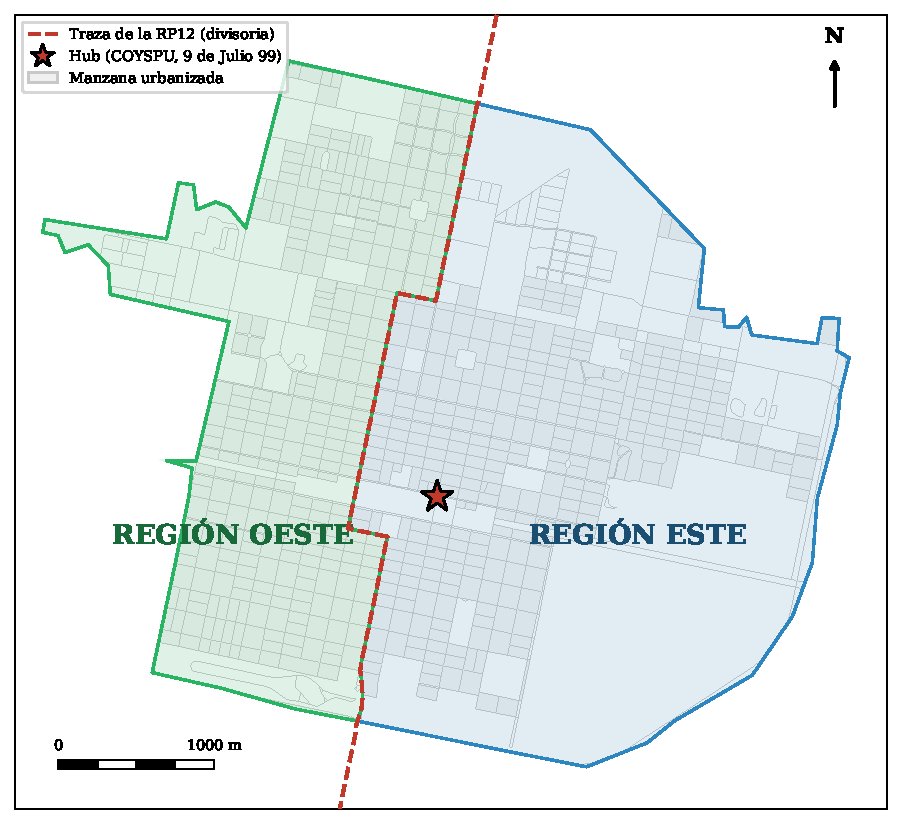
\includegraphics[height=0.72\textheight]{plano_regiones.pdf}
    \end{column}
  \end{columns}
  \note{\textbf{Cristian Arteaga Barrera:} La Parte 2 es el diseño de una red FTTH GPON para Marcos Juárez, con el hub en la Cooperativa COYSPU. El área de cobertura es la que indicó la cátedra, unos 14,6 kilómetros cuadrados, y se divide en dos regiones según la traza de la ruta 12: el Este lo diseñamos Luca y yo, y el Oeste Agustín y Joaquín, con los mismos criterios. Trabajamos con datos reales: las calles de OpenStreetMap, el censo 2022 y el listado de nodos de ARSAT, y todo el diseño se hizo con scripts de Python que están en el repositorio, así que se puede reproducir.}
\end{frame}

\orador{Grupo Este}{Cristian Arteaga Barrera}
\begin{frame}{REFEFO y ARSAT}
  \begin{columns}[T]
    \begin{column}{0.55\textwidth}
      \textbf{Red Federal de Fibra Óptica}
      \begin{itemize}
        \item Lanzada en 2010 (\emph{Argentina Conectada}), operada por ARSAT
        \item Más de $34.000$ km de fibra, 13 regiones, ``km 0'' en Benavídez
        \item \textbf{1.163 localidades conectadas} (feb.\ 2026)
        \item Red de \textbf{transporte}: vende capacidad mayorista a cooperativas y pymes, no llega al domicilio
      \end{itemize}
    \end{column}
    \begin{column}{0.45\textwidth}
      \textbf{Otras actividades de ARSAT}
      \begin{itemize}
        \item Satélites ARSAT-1 y ARSAT-2
        \item Televisión Digital Abierta
        \item Centro de datos y nube
      \end{itemize}
      \begin{block}{Para el proyecto}
        \textbf{Marcos Juárez tiene nodo REFEFO activo}: la COYSPU puede contratar ahí el tránsito IP.
      \end{block}
    \end{column}
  \end{columns}
  \note{\textbf{Cristian Arteaga Barrera:} La REFEFO es la red troncal de fibra del Estado, que opera ARSAT desde 2010. Tiene más de 34.000 km y, según los datos abiertos de ARSAT, 1.163 localidades conectadas. Lo importante es que es una red de transporte: llega a un nodo en cada localidad y ahí vende capacidad a cooperativas y pymes, que construyen la red de acceso. ARSAT además opera los satélites, la televisión digital abierta y un centro de datos. Para nuestro proyecto el dato clave es que Marcos Juárez tiene un nodo REFEFO activo, así que la cooperativa puede contratar ahí la conectividad mayorista.}
\end{frame}

\orador{Grupo Este}{Cristian Arteaga Barrera}
\begin{frame}{Fundamentos: los cinco videos de la cátedra}
  \small
  \begin{enumerate}
    \item \textbf{Reflexión interna total:} láser y fluoresceína; más allá del ángulo límite el haz avanza por reflexiones sucesivas.
    \item \textbf{Fabricación:} deposición de silicio y germanio dentro de un tubo a $\approx 2000\,^\circ$C, preforma y estirado a $125\ \mu$m.
    \item \textbf{Cables (Siemens):} fibras coloreadas, tubo holgado con sobrelongitud, tendido en ductos y empalme por fusión.
    \item \textbf{Cables submarinos:} el 97\,\% del tráfico de Internet viaja por ellos; los satélites quedan para lugares aislados.
    \item \textbf{Cómo entra Internet al país:} amarre en Las Toninas y venta a mayoristas y operadores locales.
  \end{enumerate}
  \begin{block}{Relevancia para el diseño}
    Radio de curvatura (fibra G.657 en drops), atenuación por longitud de onda (presupuesto), colores y empalme por fusión (cableado) y dependencia de la conectividad mayorista.
  \end{block}
  \note{\textbf{Cristian Arteaga Barrera:} Los cinco videos recorren toda la cadena: el principio físico de la reflexión interna total; la fabricación de la fibra por deposición dentro de un tubo y el estirado de la preforma hasta 125 micrones; la construcción del cable, con fibras coloreadas en tubos holgados; los cables submarinos, por donde pasa el 97 por ciento del tráfico de Internet; y cómo entra Internet al país por Las Toninas. Todo esto se aplica al diseño: por el radio de curvatura usamos fibra G.657 en los drops, la atenuación por longitud de onda define el presupuesto, el código de colores y el empalme por fusión se usan en el cableado, y la red de acceso depende de la conectividad mayorista.}
\end{frame}

\orador{Grupo Este}{Cristian Arteaga Barrera}
\begin{frame}{Cables submarinos en Las Toninas}
  \begin{columns}[T]
    \begin{column}{0.56\textwidth}
      \scriptsize
      \begin{tabular}{llr}
        \toprule
        \textbf{Sistema} & \textbf{Destino} & \textbf{Año} \\
        \midrule
        Firmina & Brasil, Uruguay, EE.\,UU. & 2025 \\
        Malbec & Brasil & 2021 \\
        Tannat & Brasil, Uruguay & 2018 \\
        Bicentenario & Uruguay & 2011 \\
        SAm-1 & Sudamérica, EE.\,UU. & 2001 \\
        SAC & Sudamérica, EE.\,UU. & 2000 \\
        Unisur & Uruguay & 1995 \\
        \bottomrule
      \end{tabular}\\[0.1cm]
      Fuente: TeleGeography (oct.\ 2026).
    \end{column}
    \begin{column}{0.44\textwidth}
      \begin{itemize}
        \item \textbf{Siete sistemas} en servicio
        \item Largos (SAm-1, SAC, Firmina): conexión con EE.\,UU.
        \item Cortos: Uruguay y Brasil
        \item Diversidad de rutas = \textbf{redundancia}
      \end{itemize}
      \begin{block}{Cadena completa}
        Abonado $\rightarrow$ red FTTH $\rightarrow$ hub $\rightarrow$ nodo REFEFO $\rightarrow$ troncal nacional $\rightarrow$ Las Toninas
      \end{block}
    \end{column}
  \end{columns}
  \note{\textbf{Cristian Arteaga Barrera:} En Las Toninas amarran siete sistemas, todos en servicio según el mapa de TeleGeography. Los largos, como SAm-1, SAC y Firmina, nos conectan con Estados Unidos, y los cortos con Uruguay y Brasil; tener varias rutas da redundancia ante cortes. Nuestra red es el último eslabón de esa cadena: el tráfico de un abonado va por la red FTTH hasta el hub, de ahí al nodo REFEFO, por la troncal nacional y, si va al exterior, por estos cables. Le paso a Luca, que sigue con los componentes.}
\end{frame}

\orador{Grupo Este}{Luca Baccino}
\begin{frame}{Selección de componentes}
  \small
  \begin{columns}[T]
    \begin{column}{0.5\textwidth}
      \textbf{Cables Lightera (tendido aéreo)}
      \begin{itemize}
        \item Troncal: \textbf{AS80-S TS} 24 a 144 F, G.652.D
        \item Distribución: \textbf{MINI-RA} 24 y 12 F, $7{,}2$ mm
        \item Acometida: \textbf{drop Fig.\,8} G.657.A
        \item Cruces en ducto: CFOA-SM-DD
      \end{itemize}
      \textbf{Pasivos Lightera}
      \begin{itemize}
        \item ODF DIO B144, caja FK-CEO-4M
        \item Splitter PLC 1:4 ($\leq 7{,}1$ dB)
        \item CTO FK-CTO-16MC con 1:16 ($\leq 13{,}7$ dB)
        \item Conectores SC/APC ($\leq 0{,}3$ dB)
      \end{itemize}
    \end{column}
    \begin{column}{0.5\textwidth}
      \textbf{Activos VSOL}
      \begin{itemize}
        \item OLT \textbf{V1600G2-B}: 16 PON, 4 SFP+ de 10 GE
        \item SFP \textbf{Clase C+}: Tx $+3/+7$ dBm, $S_r=-30$ dBm
        \item ONT \textbf{V2802RH}: Tx $0/+4$ dBm, $S_r=-27$ dBm
        \item Overlay: ONT V2802GWT y EDFA de $+19$ dBm
      \end{itemize}
      \begin{block}{Criterio}
        Aéreo sobre la postería: más barato y rápido que canalizar. Vanos urbanos de 30 a 50 m, cables para 80 m.
      \end{block}
    \end{column}
  \end{columns}
  \note{\textbf{Luca Baccino:} Para los pasivos usamos Lightera y para los activos VSOL, dos de los fabricantes que sugirió la cátedra. El tendido es aéreo sobre la postería, porque es mucho más barato y rápido que canalizar, y los vanos urbanos de 30 a 50 metros entran en cables para 80 metros. El troncal es AS80-S TS de 24 a 144 fibras; la distribución, MINI-RA de 24 y 12 fibras, que es muy liviano; y la acometida, drop figura 8 con fibra G.657. En activos, la OLT V1600G2-B de 16 puertos con módulos Clase C+, cuya necesidad vamos a ver en el presupuesto, y la ONT V2802RH. Todos los conectores son SC/APC, para dejar abierta la opción de video por RF.}
\end{frame}

\orador{Grupo Este}{Luca Baccino}
\begin{frame}{Laboratorio: prácticas de instalación (TP3)}
  \begin{columns}[c]
    \begin{column}{0.27\textwidth}
      \centering
      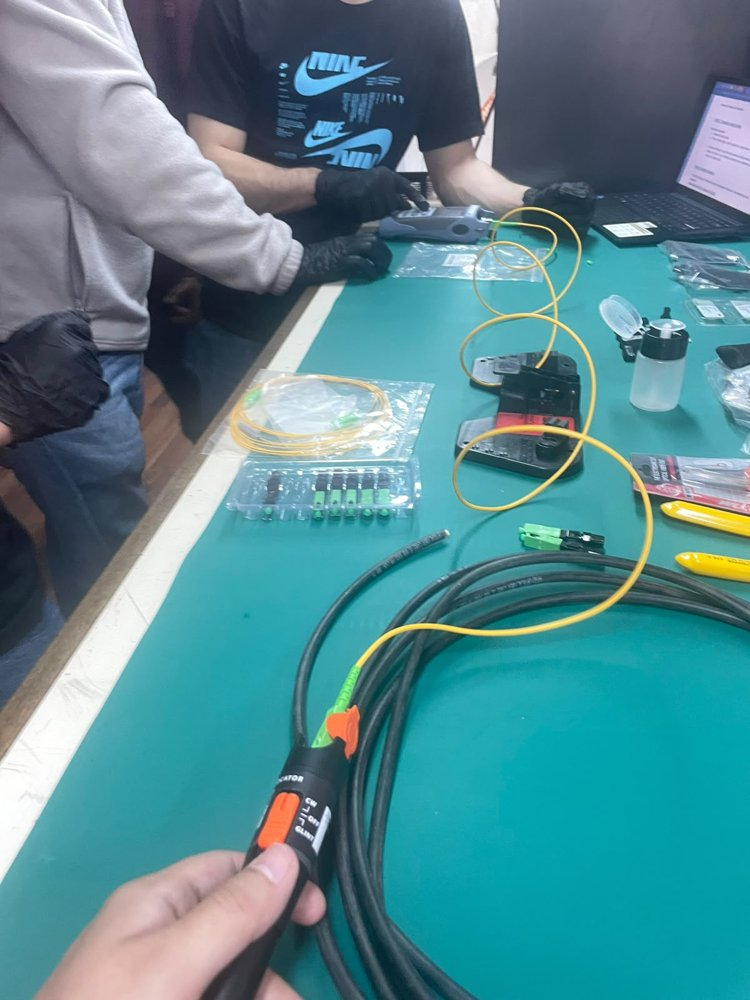
\includegraphics[height=0.42\textheight]{lab_vfl_continuidad.jpg}\\[0.05cm]
      \scriptsize VFL y medidor
    \end{column}
    \begin{column}{0.25\textwidth}
      \centering
      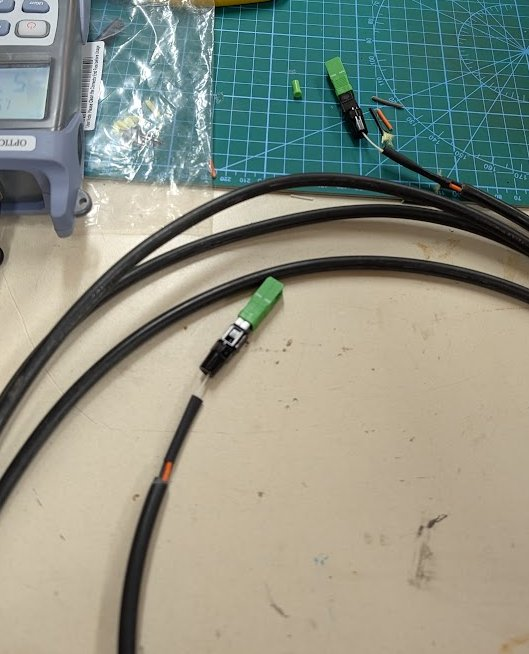
\includegraphics[height=0.42\textheight]{lab_conector_sc_apc.jpg}\\[0.05cm]
      \scriptsize Conector SC/APC
    \end{column}
    \begin{column}{0.46\textwidth}
      \small
      \begin{itemize}
        \item \textbf{VFL:} continuidad; el medidor no mide bien a 650 nm (calibrado desde 800 nm)
        \item \textbf{Conector y empalme mecánico:} varios intentos; sin potencia por una rotura del cable
      \end{itemize}
      \begin{block}{Lo que aplicamos al diseño}
        \footnotesize Empalmes por fusión en planta externa, rulos de reserva y margen de 3 dB, medidor calibrado en 1310/1490/1550 nm y OTDR para certificar.
      \end{block}
    \end{column}
  \end{columns}
  \note{\textbf{Luca Baccino:} En el laboratorio, que documentamos en el TP3, hicimos tres prácticas: verificación de continuidad con el VFL, armado de un conector mecánico SC/APC y un empalme mecánico. Aprendimos tres cosas que llevamos al diseño. El medidor no da una lectura válida fuera de su longitud de onda de calibración, así que hay que usar uno calibrado en las de la red. La fibra es muy frágil: después de varios intentos el enlace quedó sin potencia por una rotura que el VFL no pudo ubicar dentro del cable; por eso usamos empalmes por fusión, dejamos rulos de reserva y un margen de 3 dB, y proponemos certificar con OTDR.}
\end{frame}

\section[P2: Alcance]{Alcance y arquitectura}
\orador{Grupo Este}{Luca Baccino}
\begin{frame}{Casas pasadas y abonados}
  \begin{columns}[T]
    \begin{column}{0.52\textwidth}
      \small
      \begin{itemize}
        \item Censo 2022: \textbf{12.135 viviendas}
        \item Manzanas urbanizadas: entre $0{,}25$ y $2{,}5$ ha y menos del 50\,\% de usos no residenciales
        \item Densidad uniforme: $17$ viv/ha, viviendas sobre el frente de cada manzana
      \end{itemize}
      \vspace{0.1cm}
      \footnotesize
      \begin{tabular}{lrrr}
        \toprule
        & \textbf{Este} & \textbf{Oeste} & \textbf{Total} \\
        \midrule
        Casas pasadas & 6.153 & 5.982 & 12.135 \\
        1.ª etapa (45\,\%) & 2.771 & 2.697 & 5.468 \\
        Final (90\,\%) & 5.541 & 5.388 & 10.929 \\
        \bottomrule
      \end{tabular}
    \end{column}
    \begin{column}{0.48\textwidth}
      \small
      \textbf{Servicios}
      \begin{itemize}
        \item Planes de 100, 300 y 600 Mbps (30/50/20\,\%), subida 10\,\%
        \item TV y telefonía sobre IP
      \end{itemize}
      \textbf{Crecimiento y reserva}
      \begin{itemize}
        \item Red pasiva construida para la cobertura final
        \item Una fibra de crecimiento por sector
        \item Fibras dedicadas a instituciones y plazas
      \end{itemize}
      \footnotesize El 45\,\% se apoya en los $\approx 4.500$ usuarios ADSL que tuvo la COYSPU.
    \end{column}
  \end{columns}
  \note{\textbf{Luca Baccino:} Las casas pasadas salen del censo 2022: 12.135 viviendas. Como no hay datos por manzana, las repartimos en forma uniforme sobre las manzanas urbanizadas, que son las que miden entre un cuarto de hectárea y dos hectáreas y media y no están ocupadas mayormente por campos, industrias, parques, escuelas u hospitales. Resultan 6.153 casas pasadas en el Este y 5.982 en el Oeste. Suponemos una adopción del 45 por ciento el primer año, que es exigente pero razonable porque la cooperativa llegó a tener unos 4.500 usuarios de ADSL, y del 90 por ciento en la cobertura final. Los planes son de 100, 300 y 600 megas, y la red pasiva se construye desde el inicio para la cobertura final.}
\end{frame}

\orador{Grupo Este}{Luca Baccino}
\begin{frame}{Arquitectura de la red}
  \centering
  \resizebox{0.95\textwidth}{!}{%
    \begin{tikzpicture}[font=\footnotesize,
        activo/.style={draw, thick, rounded corners=2pt, fill=blue!10, minimum height=1.1cm, align=center, text width=2.1cm},
        pasivo/.style={draw, thick, fill=gray!10, minimum height=1.1cm, align=center, text width=2.1cm},
        caja/.style={draw, thick, rounded corners=5pt, fill=orange!15, minimum height=1.1cm, align=center, text width=2.1cm},
        flecha/.style={-{Stealth}, thick}]
        \node[activo] (refefo) at (0,3.2) {\textbf{Nodo REFEFO}\\ARSAT};
        \node[activo] (router) at (4.2,3.2) {\textbf{Router de borde}\\BNG, cachés};
        \node[activo] (sw) at (7.6,3.2) {\textbf{Switch de}\\\textbf{agregación}};
        \node[activo] (olt) at (11.0,3.2) {\textbf{OLT}\\V1600G2-B\\SFP Clase C+};
        \node[pasivo] (odf) at (14.4,3.2) {\textbf{ODF}\\DIO B144};
        \draw[flecha] (refefo) -- node[above, font=\scriptsize]{100GBASE-LR4} (router);
        \draw[flecha] (router) -- (sw);
        \draw[flecha] (sw) -- node[above, font=\scriptsize]{$4 \times 10G$} (olt);
        \draw[flecha] (olt) -- (odf);
        \node[caja] (ceo) at (14.4,0) {\textbf{CEO de cluster}\\FK-CEO-4M};
        \node[caja] (cd) at (11.0,0) {\textbf{Caja de distrib.}\\splitter 1:4};
        \node[caja] (cto) at (7.6,0) {\textbf{CTO}\\splitter 1:16};
        \node[pasivo] (roseta) at (4.2,0) {\textbf{Roseta}\\SC/APC};
        \node[activo] (ont) at (0,0) {\textbf{ONT}\\V2802RH};
        \draw[flecha] (odf) -- node[right, font=\scriptsize, align=left]{Troncal\\AS80-S TS} (ceo);
        \draw[flecha] (ceo) -- node[above, font=\scriptsize]{MINI-RA 24 F} (cd);
        \draw[flecha] (cd) -- node[above, font=\scriptsize]{MINI-RA 12 F} (cto);
        \draw[flecha] (cto) -- node[above, font=\scriptsize]{Drop G.657} (roseta);
        \draw[flecha] (roseta) -- (ont);
        \draw[very thick, dashed, red!70!black, rounded corners=8pt] (12.55,4.3) -- (16.1,4.3) -- (16.1,-1.0) -- (1.75,-1.0) -- (1.75,1.05) -- (12.55,1.05) -- cycle;
        \node[red!70!black, font=\small\bfseries] at (8.6,1.35) {ODN};
    \end{tikzpicture}}
  \vspace{0.15cm}

  \footnotesize
  \begin{tabular}{lll}
    \toprule
    \textbf{Unidad} & \textbf{Definición} & \textbf{Capacidad} \\
    \midrule
    Sector & 1 puerto PON: splitter 1:4 + 4 CTO 1:16 (\textbf{1:64}) & Hasta 68 viviendas \\
    Cluster & Hasta 8 sectores, bloque de \textbf{24 fibras} del troncal & 439 a 543 viviendas \\
    Área de CTO & Caja terminal de 16 salidas & Hasta 17 viviendas \\
    \bottomrule
  \end{tabular}
  \note{\textbf{Luca Baccino:} Este es el diagrama general. Del nodo REFEFO se llega al router de borde del hub, al switch de agregación y a las OLT; de ahí, por el ODF, sale la red pasiva: el troncal hasta la caja de empalme de cada cluster, el cable de cluster hasta la caja de distribución de cada sector, donde está el splitter 1:4, la distribución hasta las cajas terminales con el splitter 1:16, y el drop hasta la vivienda. La división en dos niveles da 1:64 y hace que el troncal necesite una sola fibra por sector. Las unidades de diseño son el sector, que es un puerto PON con hasta 68 viviendas; el cluster, de hasta 8 sectores con un bloque de 24 fibras; y el área de cada caja terminal, de hasta 17 viviendas.}
\end{frame}

\orador{Grupo Este}{Luca Baccino}
\begin{frame}{Región Este: sectores y troncal}
  \begin{columns}[c]
    \begin{column}{0.5\textwidth}
      \centering
      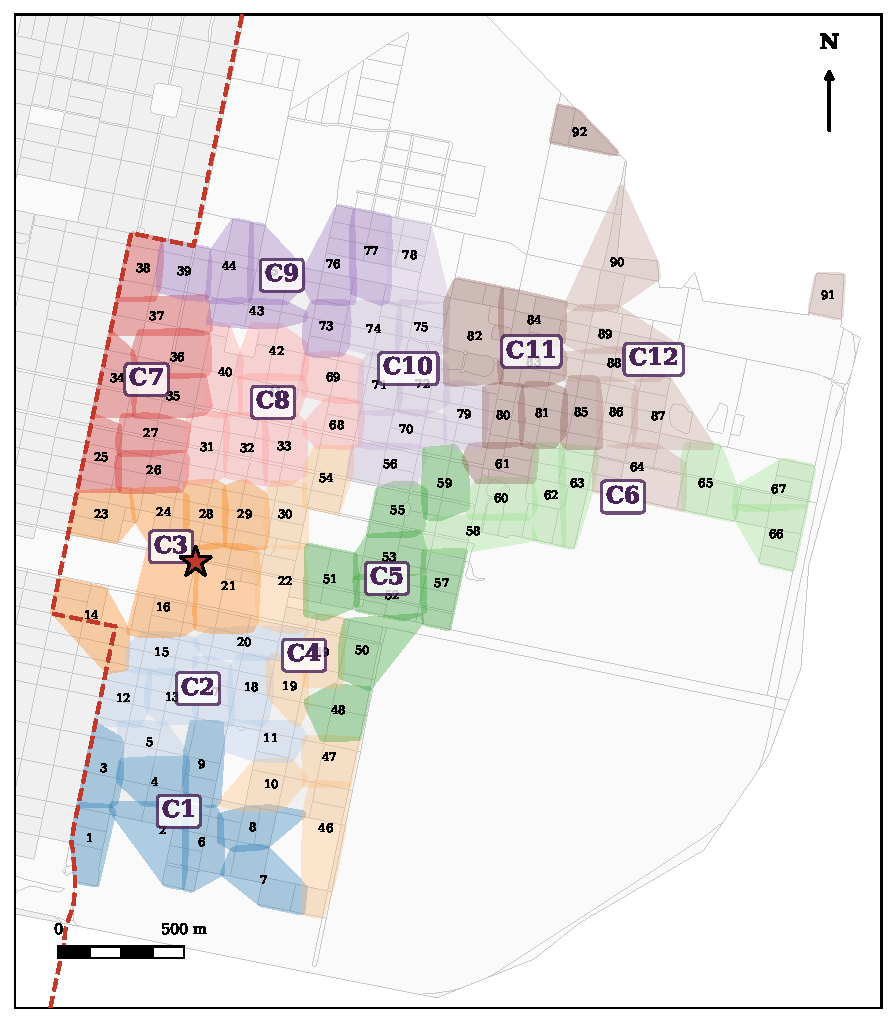
\includegraphics[height=0.78\textheight]{plano_este_sectores.pdf}
    \end{column}
    \begin{column}{0.5\textwidth}
      \centering
      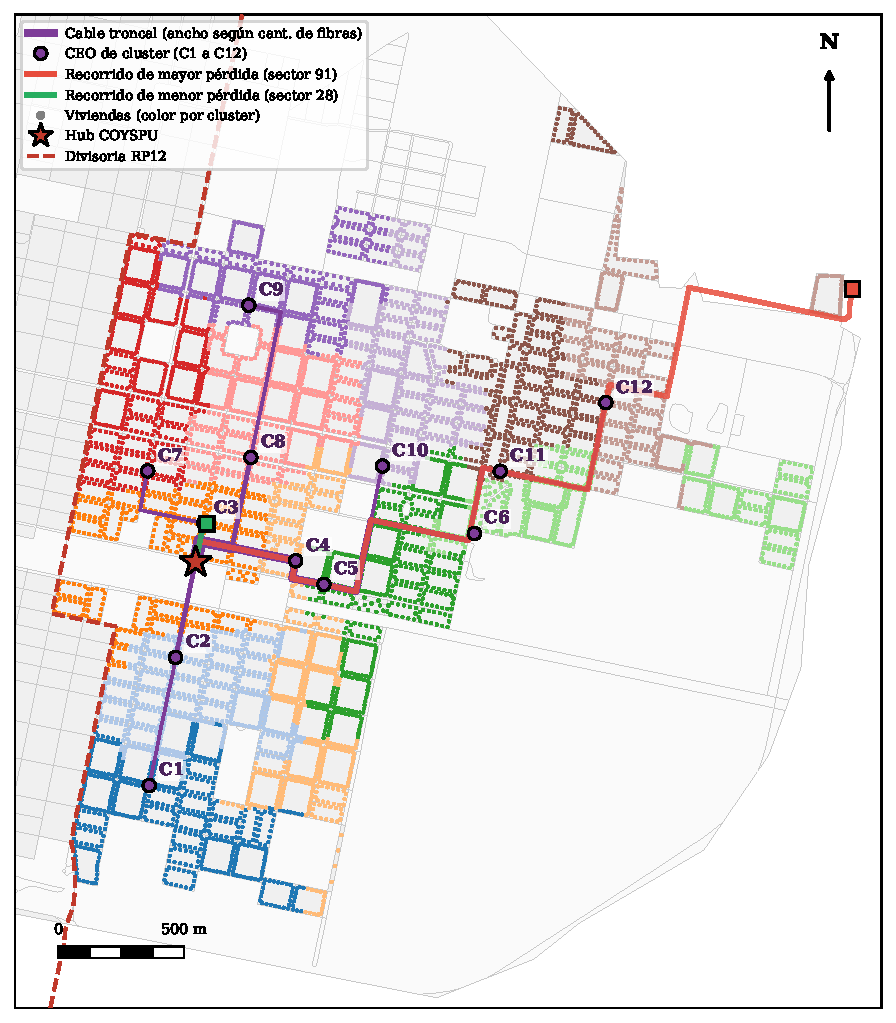
\includegraphics[height=0.78\textheight]{plano_este_troncal.pdf}
    \end{column}
  \end{columns}
  \note{\textbf{Luca Baccino:} En la Región Este quedaron 12 clusters, 92 sectores y 365 cajas terminales. Los sectores se obtuvieron por bisecciones sucesivas sobre las viviendas, y cada cluster agrupa hasta 8 sectores contiguos. A la derecha está el troncal: 5,3 km de traza que salen del hub por 9 de Julio. En verde está el recorrido de menor pérdida, junto al hub, y en rojo el de mayor pérdida, que llega al barrio aislado del noreste. La acometida media es de 68 metros.}
\end{frame}

\orador{Grupo Este}{Luca Baccino}
\begin{frame}{Región Este: sectores desarrollados}
  \begin{columns}[c]
    \begin{column}{0.36\textwidth}
      \centering
      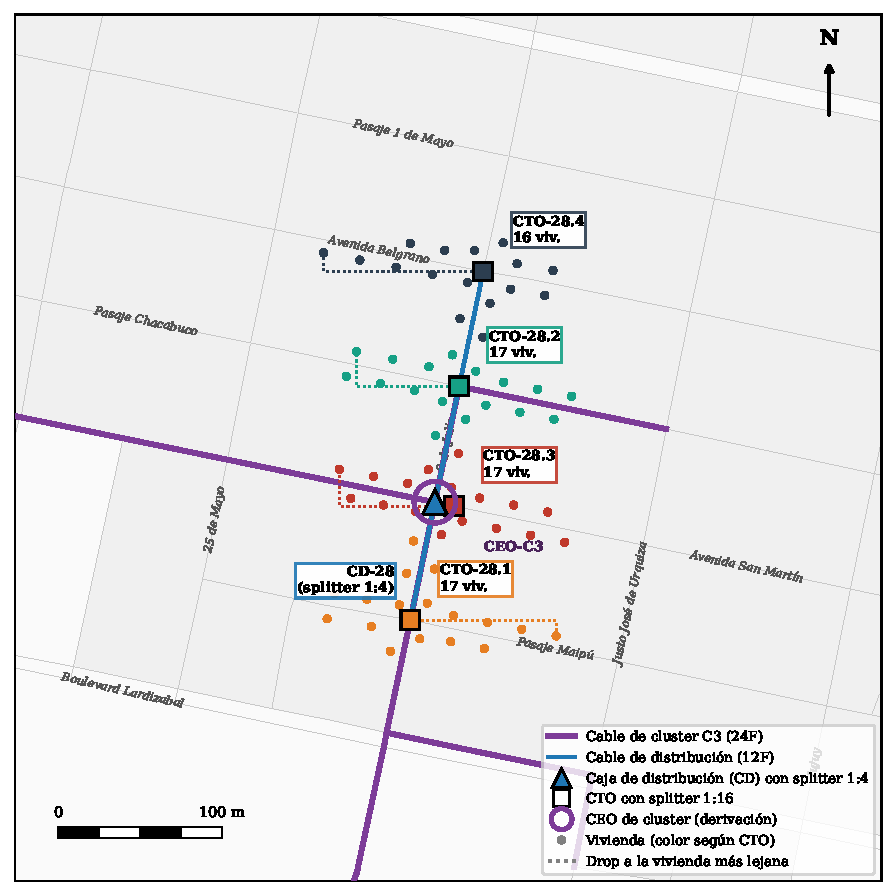
\includegraphics[width=\textwidth]{plano_sector_28.pdf}\\
      \scriptsize Sector 28 (cluster C3)
    \end{column}
    \begin{column}{0.36\textwidth}
      \centering
      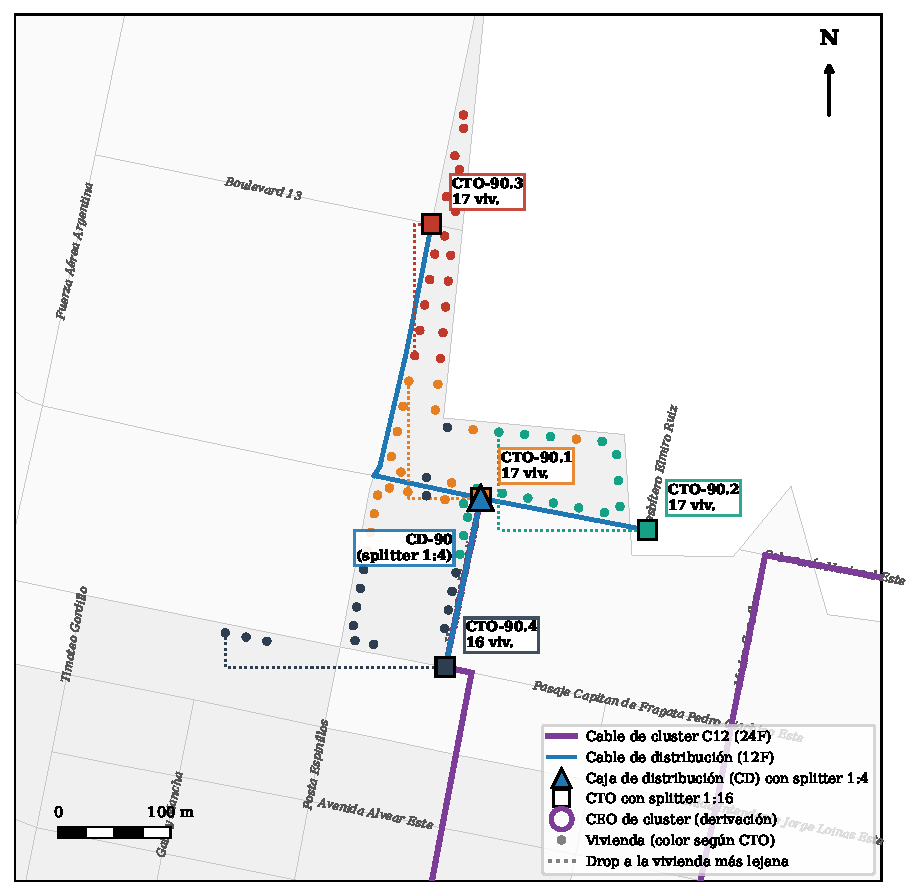
\includegraphics[width=\textwidth]{plano_sector_90.pdf}\\
      \scriptsize Sector 90 (cluster C12)
    \end{column}
    \begin{column}{0.28\textwidth}
      \scriptsize
      \textbf{Sector 28}: 67 viviendas en el centro; caja de distribución en el mismo poste que la CEO de C3; distribución de 230 m, drop máx.\ 109 m.\\[0.2cm]
      \textbf{Sector 90}: 67 viviendas en la periferia noreste, a 3,1 km del hub; distribución de 633 m, drop máx.\ 227 m.\\[0.2cm]
      Totales Este: troncal 5,29 km, cluster 26,25 km, distribución 33,40 km.
    \end{column}
  \end{columns}
  \note{\textbf{Luca Baccino:} Desarrollamos en detalle dos sectores del Este. El sector 28 está en el centro, junto al hub, y su caja de distribución coincide con la caja de empalme del cluster, así que las dos funciones se resuelven en una sola caja; tiene 230 metros de distribución. El sector 90 está en la periferia noreste, a 3,1 km del hub, y por la menor densidad necesita 633 metros de distribución y una acometida de hasta 227 metros, que habría que revisar en campo. Con esto termina la parte del Grupo Este; le paso a Agustín, que presenta la Región Oeste.}
\end{frame}

\orador{Grupo Oeste}{Agustín Mendes Rosa}
\begin{frame}{Región Oeste: sectores}
  \begin{columns}[c]
    \begin{column}{0.48\textwidth}
      \centering
      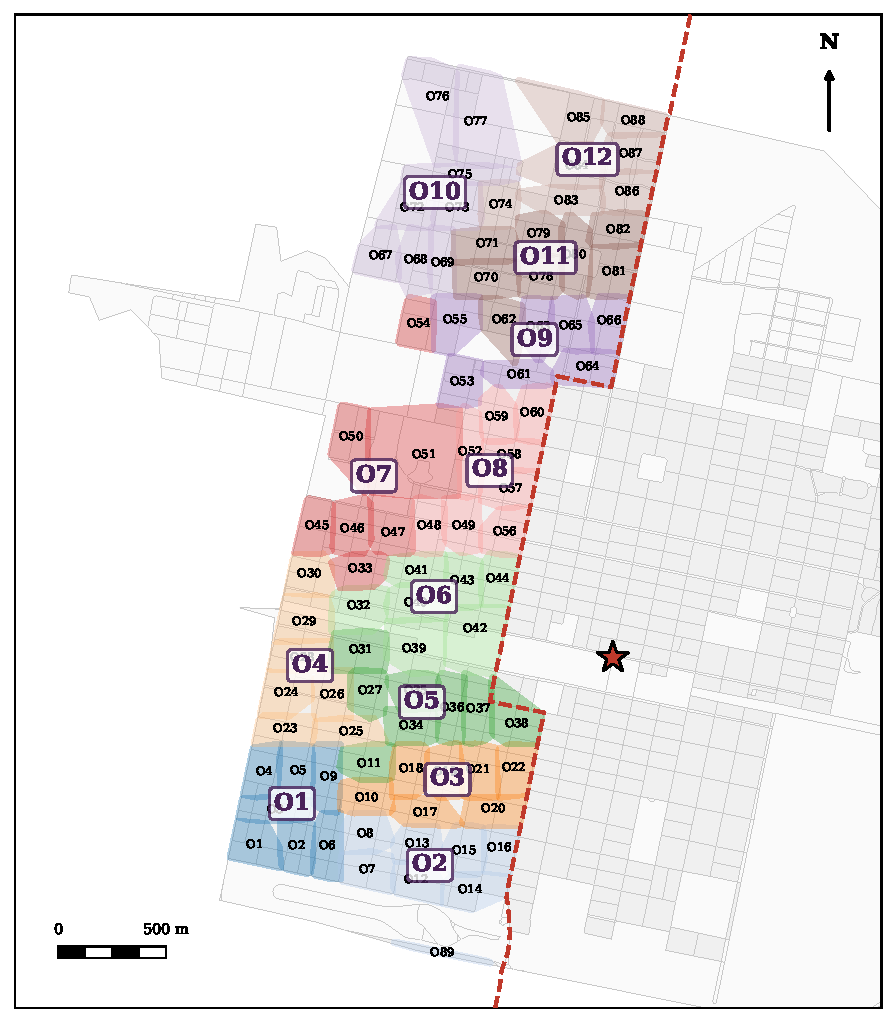
\includegraphics[height=0.8\textheight]{plano_oeste_sectores.pdf}
    \end{column}
    \begin{column}{0.52\textwidth}
      \begin{itemize}
        \item 5.982 casas pasadas
        \item \textbf{12 clusters, 89 sectores, 354 CTO}
        \item Mismos criterios que el Este
        \item Prefijo O: clusters O1--O12, sectores O1--O89
        \item Cluster de cable: 22,82 km; distribución: 32,02 km
        \item Drop medio de 69 m
      \end{itemize}
      \begin{block}{Particularidad}
        El hub está \textbf{fuera} de la región: todos los cables cruzan la RP12.
      \end{block}
    \end{column}
  \end{columns}
  \note{\textbf{Agustín Mendes Rosa:} Gracias, Luca. La Región Oeste tiene 5.982 casas pasadas y quedó organizada en 12 clusters, 89 sectores y 354 cajas terminales, con los mismos criterios que el Este. Para distinguir los elementos les agregamos el prefijo O. La particularidad es que el hub queda del lado Este, así que todos los cables del Oeste cruzan la ruta 12, y la región se extiende bastante hacia el noroeste y el sur.}
\end{frame}

\orador{Grupo Oeste}{Agustín Mendes Rosa}
\begin{frame}{Troncal: reaprovechar el cable tendido}
  \begin{columns}[c]
    \begin{column}{0.46\textwidth}
      \centering
      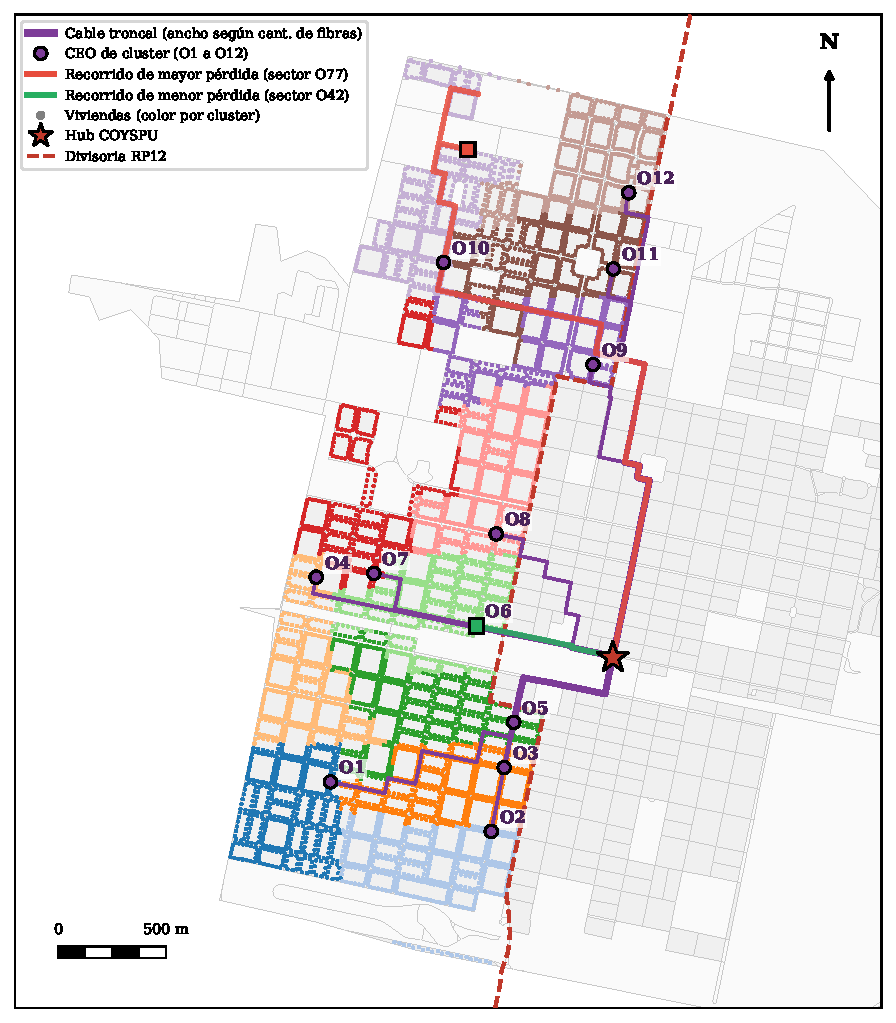
\includegraphics[height=0.8\textheight]{plano_oeste_troncal.pdf}
    \end{column}
    \begin{column}{0.54\textwidth}
      \small
      \textbf{Corrección de la cátedra:} el ramal a O8 doblaba en muchas calles.
      \begin{block}{Nuevo criterio de trazado}
        \footnotesize
        \begin{itemize}
          \item Cada cluster se deriva del \textbf{troncal ya tendido}
          \item Cada giro ($>35^\circ$) cuesta como 150 m de cable
        \end{itemize}
      \end{block}
      O8 ahora sale de la CEO de O6 y \textbf{sube derecho por Santiago del Estero}, que sigue hasta DO3 (O9 a O12).\\[0.15cm]
      \footnotesize
      \begin{tabular}{lrr}
        \toprule
        \textbf{Troncal} & \textbf{Antes} & \textbf{Ahora} \\
        \midrule
        Este & 7,22 km & 5,29 km \\
        Oeste & 10,50 km & 6,73 km \\
        \bottomrule
      \end{tabular}
    \end{column}
  \end{columns}
  \note{\textbf{Agustín Mendes Rosa:} Acá aplicamos la corrección que nos hizo la cátedra. Antes cada cluster tenía su propio camino mínimo desde el hub, y el ramal a O8 zigzagueaba por muchas calles, lo que en la práctica es más difícil y caro de tender. Cambiamos el criterio: el troncal se arma como un árbol que reaprovecha el cable ya tendido, y cada giro se penaliza como si fueran 150 metros de cable. Ahora O8 se deriva de la caja de O6 y sube derecho por Santiago del Estero, y esa misma calle lleva el troncal hasta la derivación de los clusters del norte. Aplicado a las dos regiones, el troncal bajó de 7,2 a 5,3 km en el Este y de 10,5 a 6,7 km en el Oeste.}
\end{frame}

\orador{Grupo Oeste}{Agustín Mendes Rosa}
\begin{frame}{Región Oeste: sectores desarrollados}
  \begin{columns}[c]
    \begin{column}{0.36\textwidth}
      \centering
      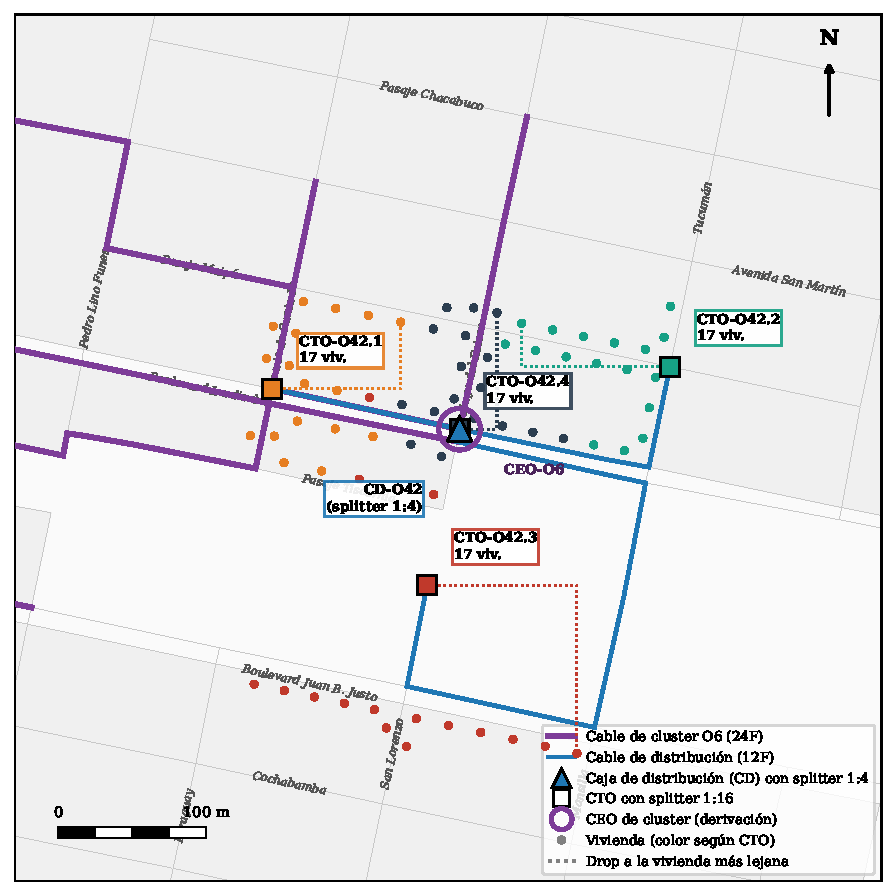
\includegraphics[width=\textwidth]{plano_sector_O42.pdf}\\
      \scriptsize Sector O42 (cluster O6)
    \end{column}
    \begin{column}{0.36\textwidth}
      \centering
      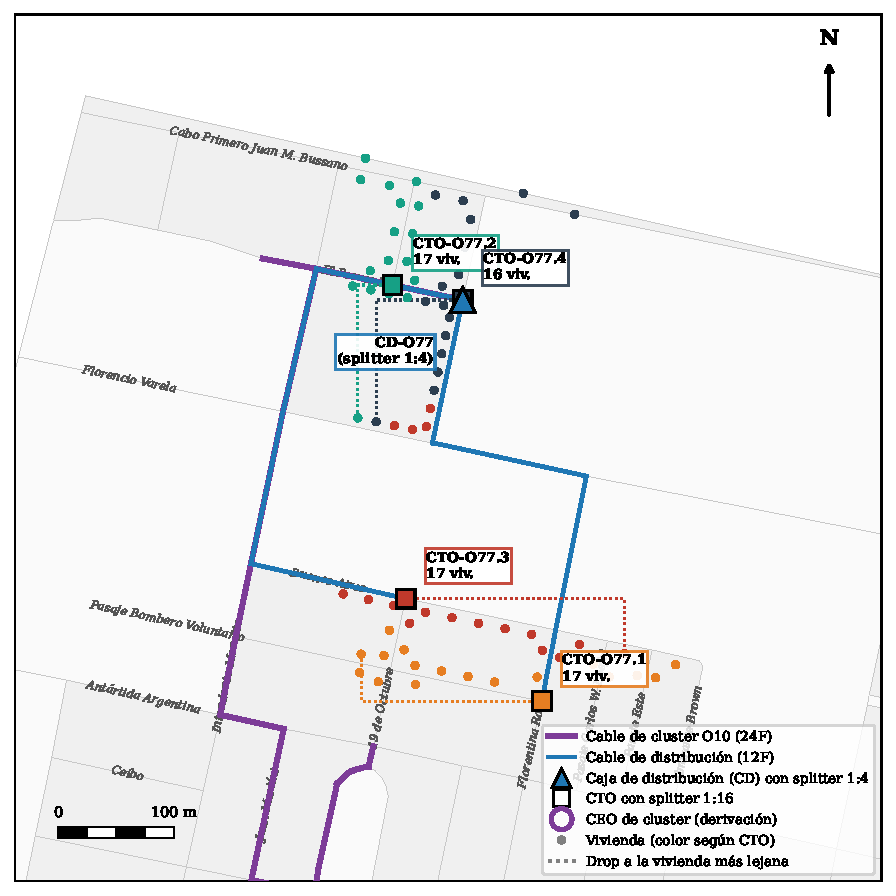
\includegraphics[width=\textwidth]{plano_sector_O77.pdf}\\
      \scriptsize Sector O77 (cluster O10)
    \end{column}
    \begin{column}{0.28\textwidth}
      \scriptsize
      \textbf{Sector O42}: 68 viviendas sobre Bv.\ Lardizábal; caja de distribución en la CEO de O6, a 664 m del hub; recorrido de \textbf{menor pérdida} del Oeste.\\[0.2cm]
      \textbf{Sector O77}: 67 viviendas en el noroeste, a 3,85 km del hub; distribución de 991 m; la CTO-O77.3 es el recorrido de \textbf{mayor pérdida}.
    \end{column}
  \end{columns}
  \note{\textbf{Agustín Mendes Rosa:} En el Oeste desarrollamos el sector O42, sobre el bulevar Lardizábal, cuya caja de distribución está en el mismo poste que la caja del cluster O6, a 664 metros del hub, y que contiene el recorrido de menor pérdida de la región. Y el sector O77, en el noroeste, a 3,85 km del hub, con 991 metros de distribución; su caja terminal O77.3 es el recorrido de mayor pérdida del Oeste, que después usa Joaquín en el presupuesto óptico.}
\end{frame}

\section[P2: Dimension.]{Dimensionamiento}
\orador{Grupo Oeste}{Agustín Mendes Rosa}
\begin{frame}{Instituciones y plazas con fibra dedicada}
  \begin{columns}[T]
    \begin{column}{0.55\textwidth}
      \small
      \begin{itemize}
        \item \textbf{27 instituciones}: escuelas, salud, policía, bomberos, municipalidad, tribunales y biblioteca
        \item \textbf{13 plazas} de al menos 1.000 m$^2$ (Wi-Fi público, cámaras)
        \item Una fibra por institución o plaza, \textbf{sin splitters}
        \item \textbf{Hospitales: 4 fibras} con un cable MINI-RA propio desde la caja de distribución
        \item Total: \textbf{49 fibras dedicadas}
      \end{itemize}
    \end{column}
    \begin{column}{0.45\textwidth}
      \begin{block}{Recorrido de la fibra dedicada}
        \footnotesize
        Troncal y cable de cluster: F17 en adelante\\
        Caja de distribución: empalme directo\\
        Distribución: fibras de reserva F9+\\
        CTO: empalme a un drop propio
      \end{block}
      \footnotesize Enlace Ethernet de 1 Gbps (1000BASE-LX): el peor caso tiene 3,64 dB de pérdida y \textbf{2,36 dB} sobre el margen.
    \end{column}
  \end{columns}
  \note{\textbf{Agustín Mendes Rosa:} Otra indicación de la cátedra fue dejar un pelo extra para las instituciones. Identificamos en OpenStreetMap 27 instituciones, entre escuelas, centros de salud, policía, bomberos, la municipalidad, tribunales y la biblioteca, y 13 plazas de al menos mil metros cuadrados. Cada una recibe una fibra propia, sin splitters, desde el ODF, y los hospitales reciben cuatro con un cable propio desde la caja de distribución. En total son 49 fibras dedicadas, que entran en las fibras libres de cada cluster y de cada cable de distribución. Con un enlace Ethernet de 1 Gbps, el caso más desfavorable conserva 2,36 dB sobre el margen.}
\end{frame}

\orador{Grupo Oeste}{Agustín Mendes Rosa}
\begin{frame}{Asignación de fibras, puertos y cantidades}
  \begin{columns}[T]
    \begin{column}{0.5\textwidth}
      \footnotesize
      \textbf{Bloque de 24 fibras de cada cluster}
      \begin{itemize}
        \item F1--F8: una por sector (al splitter 1:4)
        \item F9--F16: crecimiento
        \item F17+: instituciones y plazas
        \item Resto: reserva (al menos 2)
      \end{itemize}
      \textbf{Puertos}
      \begin{itemize}
        \item 92 + 89 = \textbf{181 puertos PON}
        \item \textbf{12 OLT} de 16 puertos (6 por región), 11 libres
        \item Splitter 1:2 en el hub: descartado (no cumple el presupuesto)
      \end{itemize}
    \end{column}
    \begin{column}{0.5\textwidth}
      \scriptsize
      \begin{tabular}{lr}
        \toprule
        \textbf{Elemento (total + 10\,\%)} & \textbf{Cantidad} \\
        \midrule
        Troncal AS80-S TS (24 a 144 F) & 14,3 km \\
        Cable de cluster MINI-RA 24 F & 54,0 km \\
        Distribución MINI-RA 12 F & 72,0 km \\
        Drops, primera etapa & 457 km \\
        \midrule
        Cajas FK-CEO-4M & 188 \\
        Splitters 1:4 & 181 \\
        CTO con splitter 1:16 & 719 \\
        ODF DIO B144 & 4 \\
        \bottomrule
      \end{tabular}
    \end{column}
  \end{columns}
  \note{\textbf{Agustín Mendes Rosa:} Cada cluster recibe un bloque de 24 fibras: las primeras ocho van una a cada sector, las ocho siguientes son de crecimiento, después vienen las de instituciones y plazas, y el resto queda de reserva. Como cada sector usa un puerto PON, la red necesita 181 puertos, que se cubren con 12 OLT de 16 puertos, seis por región, y quedan 11 libres. Evaluamos compartir puertos con un splitter 1:2 en el hub, pero el recorrido más largo dejaría de cumplir el presupuesto óptico. A la derecha está el resumen de cantidades: unos 14 km de troncal, 54 de cable de cluster, 72 de distribución, 719 cajas terminales y 457 km de drop en la primera etapa.}
\end{frame}

\orador{Grupo Oeste}{Agustín Mendes Rosa}
\begin{frame}{Identificación y continuidad óptica}
  \footnotesize
  \begin{itemize}
    \item OLT-E1..E6 y OLT-O1..O6: la OLT $n$ atiende los clusters $2n-1$ y $2n$
    \item ODF de 144 posiciones: 24 consecutivas por cluster; fibras con código de colores ABNT
    \item Tramos CT-01..CT-16 (Este) y CT-O01..CT-O15 (Oeste); cajas D1--D4 y DO1--DO3
  \end{itemize}
  \vspace{0.1cm}
  \scriptsize
  \begin{tabular}{lll}
    \toprule
    \textbf{Elemento} & \textbf{Sector 28 (C3)} & \textbf{Sector O77 (O10)} \\
    \midrule
    Puerto PON & OLT-E2, PON 6 & OLT-O5, PON 15 \\
    Posición en el ODF & ODF-E1, 54 & ODF-O2, 80 \\
    Fibra del troncal & C3-F6 (violeta) & O10-F8 (rosa) \\
    Tramos del troncal & CT-01, CT-03 & CT-O01, O02, O04, O05, O08, O13 \\
    Derivaciones & D1 & DO1, CEO-O6, DO2, CEO-O8, DO3 \\
    Caja de distribución & 9 de Julio y Av.\ San Martín & 19 de Octubre y El Porvenir \\
    Distribución & DS-28, F1--F4 & DS-O77, F1--F4 \\
    \bottomrule
  \end{tabular}
  \note{\textbf{Agustín Mendes Rosa:} Para el cableado definimos una identificación coherente con los planos y las tablas: cada OLT atiende dos clusters consecutivos, cada cluster ocupa 24 posiciones consecutivas del ODF y las fibras siguen el código de colores del fabricante. La tabla muestra la continuidad completa de dos sectores: por ejemplo, el sector O77 sale del puerto 15 de la OLT-O5, ocupa la posición 80 del ODF-O2, usa la fibra 8 del bloque de O10, que es la rosa, y recorre seis tramos del troncal pasando por cinco cajas de derivación hasta su caja de distribución. Le paso a Joaquín, que sigue con la conectividad mayorista.}
\end{frame}

\orador{Grupo Oeste}{Joaquín Monja}
\begin{frame}{Conectividad mayorista: procedimiento de la cátedra}
  \begin{columns}[T]
    \begin{column}{0.5\textwidth}
      \small
      \begin{enumerate}
        \item Suma comercial: $C_{com} = \sum N_{plan}\, v_{plan}$
        \item Simultaneidad $F_s$; overbooking $OB = 1/F_s$
        \item $C_{pico} = C_{com} \cdot F_s$
        \item $C_{obj} = C_{pico}\,(1 + M)$, con $M = 25$\,\%
      \end{enumerate}
      \textbf{Escenarios:} $F_s = 5$\,\% (diseño, 20:1) y $10$\,\% (conservador, 10:1)\\[0.15cm]
      \footnotesize El overbooking no es la división óptica 1:64.
    \end{column}
    \begin{column}{0.5\textwidth}
      \centering
      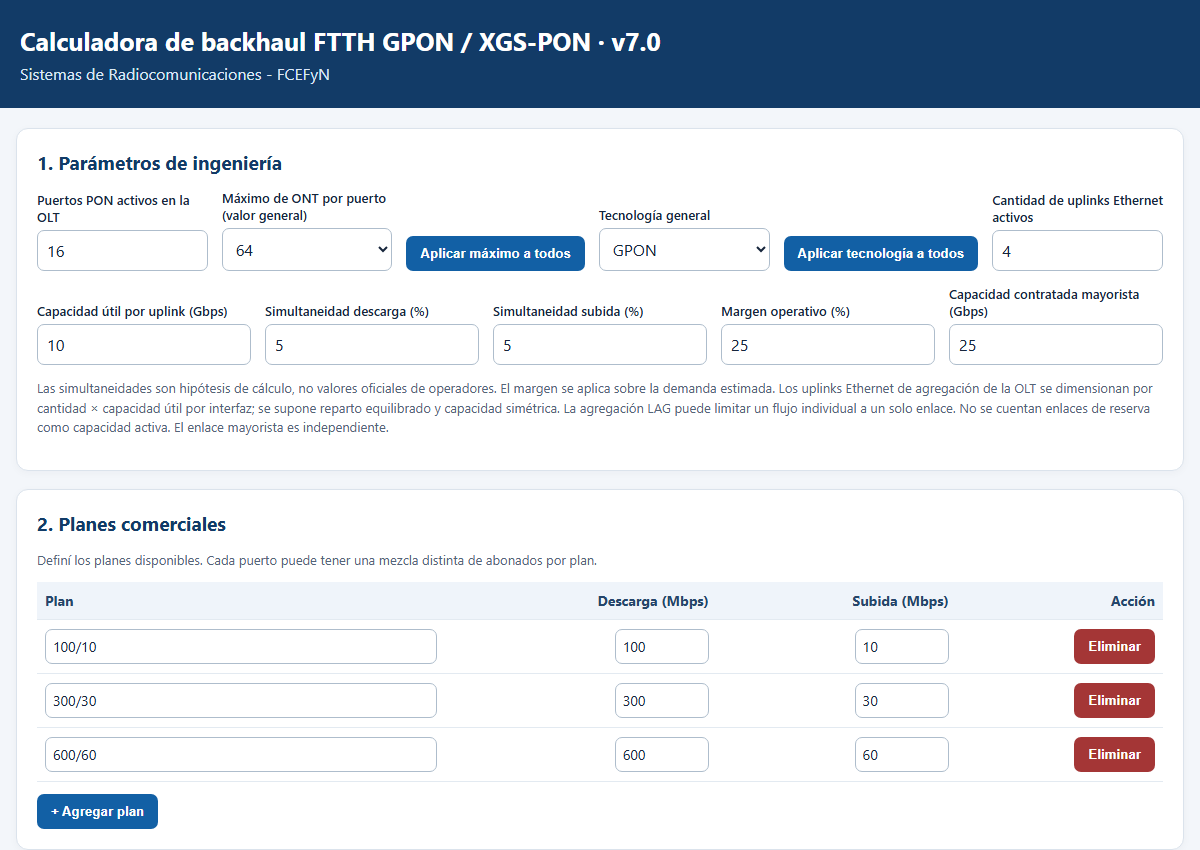
\includegraphics[width=\textwidth]{calculadora_parametros.png}\\
      \scriptsize Calculadora de la cátedra: \textbf{una configuración por OLT y etapa} (24), con los abonados reales de cada sector.
    \end{column}
  \end{columns}
  \note{\textbf{Joaquín Monja:} Gracias, Agustín. La conectividad mayorista la dimensionamos con el procedimiento y la calculadora que nos dio la cátedra. Se suma la velocidad comercial de todos los planes, se multiplica por un factor de simultaneidad, cuya inversa es el overbooking, y se agrega un margen operativo del 25 por ciento. Como la red es nueva y no hay mediciones, evaluamos los dos escenarios que recomienda la cátedra: 5 por ciento, que es overbooking 20 a 1, como diseño, y 10 por ciento como escenario conservador. La calculadora admite hasta 32 puertos, así que cargamos una configuración por OLT y por etapa, 24 en total, con los abonados reales de cada sector, y sumamos los resultados.}
\end{frame}

\orador{Grupo Oeste}{Joaquín Monja}
\begin{frame}{Resultados de la calculadora}
  \begin{columns}[T]
    \begin{column}{0.48\textwidth}
      \centering
      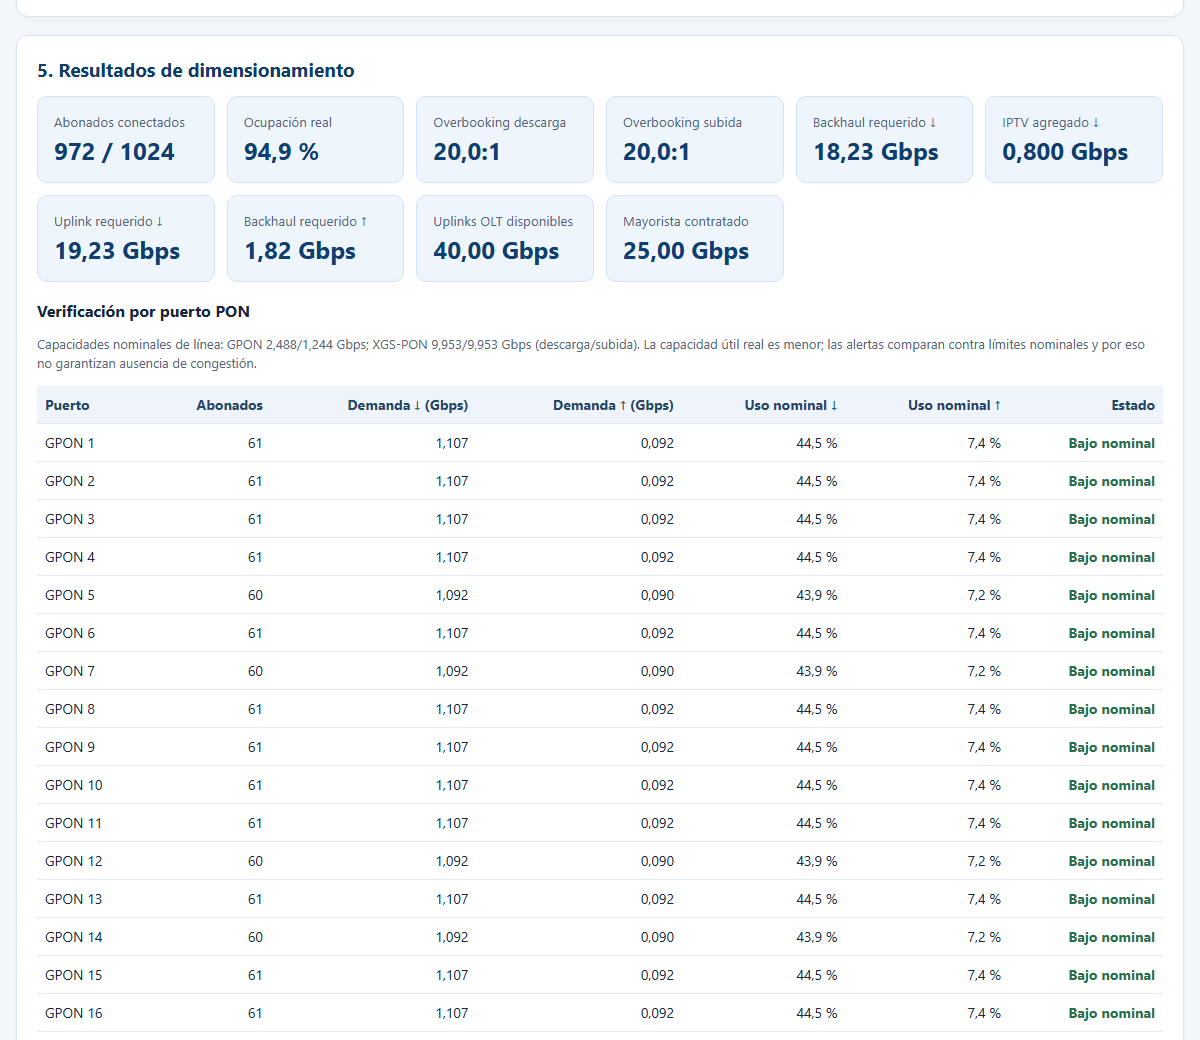
\includegraphics[width=\textwidth]{calculadora_resultados.png}\\
      \scriptsize OLT-E1, cobertura final, $F_s = 5$\,\%
    \end{column}
    \begin{column}{0.52\textwidth}
      \scriptsize
      \begin{tabular}{lrr}
        \toprule
        \textbf{Backhaul de bajada} & $F_s = 5$\,\% & $F_s = 10$\,\% \\
        \midrule
        1.ª etapa (5.468 ab.) & \textbf{102,5 Gbps} & 205 Gbps \\
        Final (10.929 ab.) & \textbf{204,9 Gbps} & 410 Gbps \\
        \bottomrule
      \end{tabular}\\[0.15cm]
      \small
      \begin{itemize}
        \item Contrato: \textbf{2$\times$100 GbE} (51\,\%), luego \textbf{3$\times$100 GbE} (68\,\%)
        \item Enlace \textbf{100GBASE-LR4}: 2,92 dB + 3 dB $\leq$ 6,3 dB
        \item Uplinks: \textbf{4$\times$10 GE por OLT} (con 2 llegaba al 96\,\%)
        \item Puertos PON: 45\,\% de uso en la cobertura final
      \end{itemize}
      \footnotesize Contraste OpenVault (5 Mbps por abonado): 34 Gbps. Permite contratar por etapas.
    \end{column}
  \end{columns}
  \note{\textbf{Joaquín Monja:} Estos son los resultados. Con la simultaneidad de diseño, la red necesita 102,5 Gbps en la primera etapa y unos 205 en la cobertura final; en el escenario conservador, el doble. Por eso proponemos contratar dos interfaces de 100 Gbps al principio, con un uso del 51 por ciento, y pasar a tres en la cobertura final. El enlace al nodo REFEFO es 100GBASE-LR4, que admite 6,3 dB y en nuestro caso tiene 2,92 más los 3 de margen. La calculadora también mostró que con dos uplinks por OLT llegábamos al 96 por ciento, así que usamos los cuatro. Como contraste, con el consumo medio de OpenVault la demanda sería tres veces menor, lo que permite contratar por etapas y ajustar con mediciones.}
\end{frame}

\section[P2: Verificación]{Verificación}
\orador{Grupo Oeste}{Joaquín Monja}
\begin{frame}{Presupuesto óptico: recorridos extremos}
  \scriptsize
  \begin{tabular}{lrrrr}
    \toprule
    & \multicolumn{2}{c}{\textbf{Mayor pérdida}} & \multicolumn{2}{c}{\textbf{Menor pérdida}} \\
    \cmidrule(lr){2-3}\cmidrule(lr){4-5}
    \textbf{Elemento} & CTO-91.1 & CTO-O77.3 & CTO-28.3 & CTO-O42.4 \\
    \midrule
    Fibra (red + drop) & 1,62 dB & 1,75 dB & 0,07 dB & 0,19 dB \\
    Splitters 1:4 y 1:16 & 20,80 dB & 20,80 dB & 18,06 dB & 18,06 dB \\
    Conexiones & 1,50 dB & 1,50 dB & 0 & 0 \\
    Empalmes & 1,30 dB & 1,10 dB & 0 & 0 \\
    \midrule
    \textbf{Pérdida total} & \textbf{25,22 dB} & \textbf{25,15 dB} & \textbf{18,13 dB} & \textbf{18,25 dB} \\
    \bottomrule
  \end{tabular}
  \vspace{0.2cm}

  \small
  \begin{columns}[T]
    \begin{column}{0.5\textwidth}
      \begin{block}{Peor caso (con $P_{t,min}$)}
        Bajada: $-22{,}22$ dBm vs.\ $S_r = -27$\\
        Subida: $-25{,}22$ dBm vs.\ $S_r = -30$\\
        Sobrante sobre $M_s$: \textbf{1,78 dB} (Este), 1,85 dB (Oeste)
      \end{block}
    \end{column}
    \begin{column}{0.5\textwidth}
      \begin{block}{Mejor caso (con $P_{t,max}$)}
        Bajada: $-11{,}13$ dBm $< -8$ dBm\\
        Subida: $-14{,}13$ dBm $< -12$ dBm\\
        Ningún receptor se satura
      \end{block}
    \end{column}
  \end{columns}
  \note{\textbf{Joaquín Monja:} El presupuesto óptico lo verificamos en los dos sentidos y en los recorridos extremos de cada región. Los de mayor pérdida son la CTO 91.1 en el Este y la O77.3 en el Oeste: los splitters se llevan casi 21 dB, y con fibra, conexiones y empalmes se llega a unos 25,2 dB. Aun así, con la potencia mínima de transmisión quedan 1,78 dB por encima del margen de 3 dB en el Este y 1,85 en el Oeste. En los recorridos más cortos, con la potencia máxima, ni la ONT ni la OLT se saturan.}
\end{frame}

\orador{Grupo Oeste}{Joaquín Monja}
\begin{frame}{Lo que justificó el presupuesto}
  \begin{itemize}
    \item \textbf{Óptica Clase C+:} con Clase B+ el peor caso no cumpliría en subida ($-0{,}22$ dB)
    \item \textbf{Un puerto por sector:} un splitter 1:2 en el hub dejaría $-2{,}22$ dB (no cumple)
    \item \textbf{Sin atenuadores} con C+; con C++ (+10 dBm) la ONT más cercana quedaría al límite de saturación
    \item \textbf{Troncal reaprovechado:} más cajas atravesadas, pero el diseño sigue cumpliendo
    \item \textbf{Video overlay:} el WDM suma 0,8 dB y todavía sobran 0,98 dB
  \end{itemize}
  \note{\textbf{Joaquín Monja:} El presupuesto justificó varias decisiones. La óptica Clase C+ es necesaria: con Clase B+ el recorrido más largo no cumpliría en subida. No conviene compartir puertos con un splitter 1:2 en el hub, porque faltarían más de 2 dB. Con C+ no hacen falta atenuadores, pero no habría que pasar a módulos C++ sin revisar los recorridos cortos. El cambio de trazado del troncal hace pasar las fibras por más cajas de derivación, pero el diseño sigue cumpliendo. Y si en el futuro se agrega video por RF, el WDM suma 0,8 dB y todavía sobra casi 1 dB.}
\end{frame}

\orador{Grupo Oeste}{Joaquín Monja}
\begin{frame}{Alternativas para distribuir televisión}
  \small
  \begin{tabular}{>{\raggedright\arraybackslash}p{2.4cm}>{\raggedright\arraybackslash}p{4.6cm}>{\raggedright\arraybackslash}p{4.4cm}}
    \toprule
    & \textbf{IPTV} & \textbf{Video overlay (1550 nm)} \\
    \midrule
    Tráfico & Multicast fijo por canal; unicast proporcional a los espectadores & RF, independiente de los espectadores \\
    Recursos & Puerto GPON; mayorista si es unicast o externa & Longitud de onda propia \\
    Equipos & Cabecera IPTV, decodificador & Transmisor, 6 EDFA, ONT con RF \\
    Presupuesto & No afecta la ODN & $-6{,}5$ dBm en el peor caso (óptimo: 0 a $-10$) \\
    \bottomrule
  \end{tabular}
  \vspace{0.2cm}
  \begin{block}{Elección: IPTV multicast con cabecera local}
    Según la calculadora: 0,19 Gbps por puerto y 0,8 Gbps por OLT, \textbf{nulo sobre el mayorista}. El overlay queda como opción para migrar la red HFC sin decodificadores.
  \end{block}
  \note{\textbf{Joaquín Monja:} Para la televisión comparamos dos alternativas. La televisión sobre IP viaja dentro de la capacidad GPON: en multicast cada canal se envía una sola vez, y en unicast cada espectador tiene su propio flujo. El video overlay transmite la grilla de RF en una tercera longitud de onda, a 1550 nm, con transmisor y amplificadores, y la ONT necesita receptor de RF; verificamos que llegan -6,5 dBm en el peor caso, dentro del rango óptimo. Elegimos IPTV multicast con cabecera local en el hub: según la calculadora consume 0,19 Gbps por puerto y nada del enlace mayorista. El overlay queda como opción si la cooperativa quiere migrar sus abonados de cable sin entregar decodificadores.}
\end{frame}

\section[Conclusiones]{Conclusiones}
\orador{Grupo Oeste}{Joaquín Monja}
\begin{frame}{Conclusiones de la Parte 2}
  \small
  \begin{itemize}
    \item Red FTTH GPON para \textbf{12.135 casas pasadas}: 24 clusters, 181 sectores, 719 CTO y 12 OLT
    \item División 1:4 + 1:16: \textbf{una fibra de troncal por sector}
    \item Troncal de \textbf{12 km} que reaprovecha el cable tendido y evita giros
    \item Presupuesto óptico: cumple en ambos sentidos con \textbf{óptica Clase C+}
    \item \textbf{49 fibras dedicadas} a instituciones, hospitales y plazas
    \item Mayorista: nodo REFEFO local, \textbf{2--3$\times$100 GbE} según la calculadora de la cátedra
    \item TV: IPTV multicast desde una cabecera local
  \end{itemize}
  \begin{block}{Limitaciones}
    \footnotesize Viviendas estimadas con densidad uniforme, cartografía de OSM, ubicación del nodo REFEFO y postería a verificar en campo, y valores de catálogo a validar con mediciones y OTDR.
  \end{block}
  \note{\textbf{Joaquín Monja:} Para cerrar: diseñamos una red FTTH GPON para las 12.135 viviendas de Marcos Juárez, con 24 clusters, 181 sectores y 12 OLT. La división en dos niveles hace que el troncal necesite una sola fibra por sector, y con el criterio de reaprovechar el cable tendido el troncal quedó en unos 12 km. El presupuesto cumple en ambos sentidos con óptica Clase C+, las instituciones y plazas tienen 49 fibras dedicadas, y la conectividad mayorista se resuelve en el nodo REFEFO local con dos a tres interfaces de 100 Gbps. Las principales limitaciones son que las viviendas se estimaron con densidad uniforme y que varios supuestos, como la postería y la ubicación del nodo, hay que verificarlos en campo. Muchas gracias.}
\end{frame}

\orador{}{}
\begin{frame}
  \centering
  \Large ¡Gracias!\\[0.4cm]
  \normalsize ¿Preguntas?
  \note{\textbf{Todos:} Quedamos a disposición para las preguntas. Cada integrante responde sobre su parte: Cristian sobre la selección de elementos y la investigación, Luca sobre el presupuesto de la Parte 1 y el diseño del Este, Agustín sobre el Oeste, el troncal y las instituciones, y Joaquín sobre la conectividad mayorista, el presupuesto óptico y la televisión.}
\end{frame}
